%
% vergleich.tex
%
% (c) 2018 Prof Dr Andreas Müller, Hochschule Rapperswil
%
\documentclass[tikz]{standalone}
\usepackage{times}
\usepackage{amsmath}
\usepackage{txfonts}
\usepackage[utf8]{inputenc}
\usepackage{graphics}
\usetikzlibrary{arrows,intersections}
\begin{document}
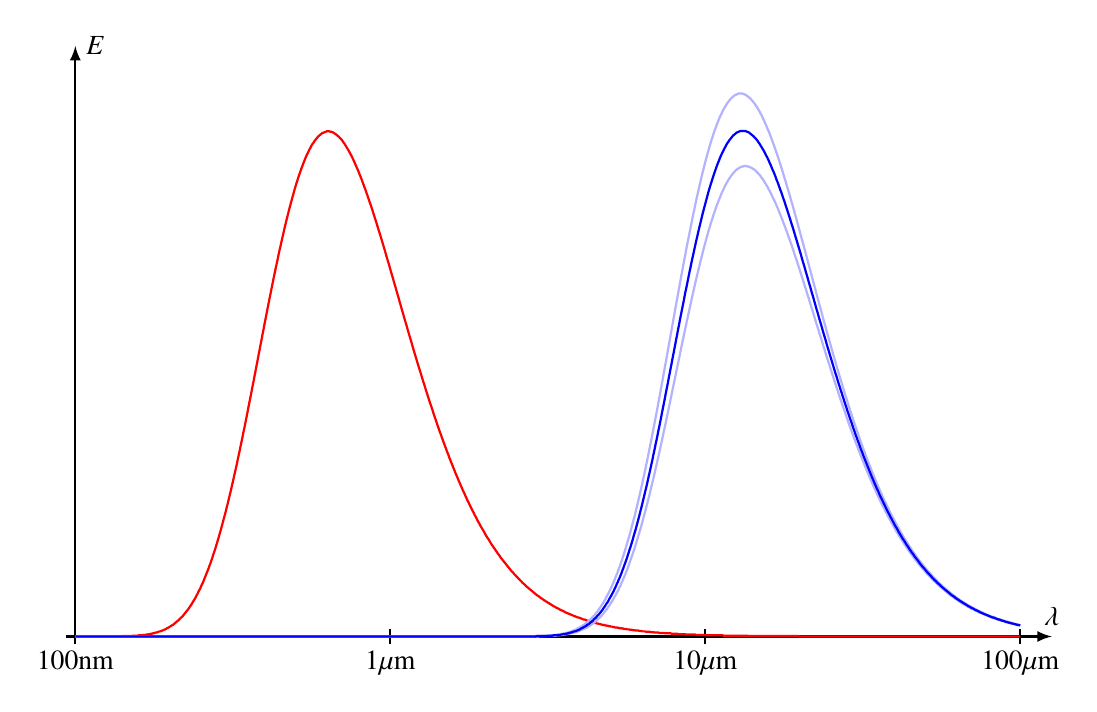
\begin{tikzpicture}[thick, >= latex, xscale=4, yscale=5]

\draw[->] (-0.03,0)--(3.1,0) coordinate[label={above:$\lambda$}];
\draw[->] (0,-0.02)--(0,1.5)
	coordinate[label={right:$E$}];
%	coordinate[label={right:$E\;[\mu\text{W}/\text{nm}\cdot\text{m}^2]$}];

\foreach \x in {0,1,...,3}{
	\draw ({\x},-0.02)--({\x},0.02);
}
%\foreach \y in {0,1,...,8}{
%	\draw (-0.02,{\y})--(0.02,{\y});
%}


\node at (0,-0.01) [below] {$100$nm};
\node at (1,-0.01) [below] {$1\mu$m};
\node at (2,-0.01) [below] {$10\mu$m};
\node at (3,-0.01) [below] {$100\mu$m};
%\node at (4,-0.1) [below] {$1$mm};

%\foreach \y in {1,2,...,8}{
%	\node at (-0.03,{\y}) [left] {$\y 0$};
%}

\draw[color=red] (0.000, 0.000)
--(0.003, 0.000)
--(0.006, 0.000)
--(0.009, 0.000)
--(0.012, 0.000)
--(0.015, 0.000)
--(0.018, 0.000)
--(0.021, 0.000)
--(0.024, 0.000)
--(0.027, 0.000)
--(0.030, 0.000)
--(0.033, 0.000)
--(0.036, 0.000)
--(0.039, 0.000)
--(0.042, 0.000)
--(0.045, 0.000)
--(0.048, 0.000)
--(0.051, 0.000)
--(0.054, 0.000)
--(0.057, 0.000)
--(0.060, 0.000)
--(0.063, 0.000)
--(0.066, 0.000)
--(0.069, 0.000)
--(0.072, 0.000)
--(0.075, 0.000)
--(0.078, 0.000)
--(0.081, 0.000)
--(0.084, 0.000)
--(0.087, 0.000)
--(0.090, 0.000)
--(0.093, 0.000)
--(0.096, 0.000)
--(0.099, 0.000)
--(0.102, 0.000)
--(0.105, 0.000)
--(0.108, 0.000)
--(0.111, 0.000)
--(0.114, 0.000)
--(0.117, 0.000)
--(0.120, 0.000)
--(0.123, 0.000)
--(0.126, 0.000)
--(0.129, 0.000)
--(0.132, 0.000)
--(0.135, 0.000)
--(0.138, 0.000)
--(0.141, 0.000)
--(0.144, 0.000)
--(0.147, 0.001)
--(0.150, 0.001)
--(0.153, 0.001)
--(0.156, 0.001)
--(0.159, 0.001)
--(0.162, 0.001)
--(0.165, 0.001)
--(0.168, 0.001)
--(0.171, 0.001)
--(0.174, 0.001)
--(0.177, 0.001)
--(0.180, 0.001)
--(0.183, 0.002)
--(0.186, 0.002)
--(0.189, 0.002)
--(0.192, 0.002)
--(0.195, 0.002)
--(0.198, 0.002)
--(0.201, 0.003)
--(0.204, 0.003)
--(0.207, 0.003)
--(0.210, 0.003)
--(0.213, 0.003)
--(0.216, 0.004)
--(0.219, 0.004)
--(0.222, 0.004)
--(0.225, 0.005)
--(0.228, 0.005)
--(0.231, 0.005)
--(0.234, 0.006)
--(0.237, 0.006)
--(0.240, 0.007)
--(0.243, 0.007)
--(0.246, 0.008)
--(0.249, 0.008)
--(0.252, 0.009)
--(0.255, 0.010)
--(0.258, 0.010)
--(0.261, 0.011)
--(0.264, 0.012)
--(0.267, 0.013)
--(0.270, 0.013)
--(0.273, 0.014)
--(0.276, 0.015)
--(0.279, 0.016)
--(0.282, 0.017)
--(0.285, 0.018)
--(0.288, 0.019)
--(0.291, 0.021)
--(0.294, 0.022)
--(0.297, 0.023)
--(0.300, 0.025)
--(0.303, 0.026)
--(0.306, 0.028)
--(0.309, 0.029)
--(0.312, 0.031)
--(0.315, 0.033)
--(0.318, 0.035)
--(0.321, 0.037)
--(0.324, 0.039)
--(0.327, 0.041)
--(0.330, 0.043)
--(0.333, 0.046)
--(0.336, 0.048)
--(0.339, 0.050)
--(0.342, 0.053)
--(0.345, 0.056)
--(0.348, 0.059)
--(0.351, 0.062)
--(0.354, 0.065)
--(0.357, 0.068)
--(0.360, 0.071)
--(0.363, 0.075)
--(0.366, 0.078)
--(0.369, 0.082)
--(0.372, 0.086)
--(0.375, 0.090)
--(0.378, 0.094)
--(0.381, 0.098)
--(0.384, 0.103)
--(0.387, 0.107)
--(0.390, 0.112)
--(0.393, 0.117)
--(0.396, 0.121)
--(0.399, 0.127)
--(0.402, 0.132)
--(0.405, 0.137)
--(0.408, 0.143)
--(0.411, 0.149)
--(0.414, 0.155)
--(0.417, 0.161)
--(0.420, 0.167)
--(0.423, 0.173)
--(0.426, 0.180)
--(0.429, 0.186)
--(0.432, 0.193)
--(0.435, 0.200)
--(0.438, 0.208)
--(0.441, 0.215)
--(0.444, 0.222)
--(0.447, 0.230)
--(0.450, 0.238)
--(0.453, 0.246)
--(0.456, 0.254)
--(0.459, 0.263)
--(0.462, 0.271)
--(0.465, 0.280)
--(0.468, 0.289)
--(0.471, 0.298)
--(0.474, 0.307)
--(0.477, 0.316)
--(0.480, 0.326)
--(0.483, 0.335)
--(0.486, 0.345)
--(0.489, 0.355)
--(0.492, 0.365)
--(0.495, 0.375)
--(0.498, 0.386)
--(0.501, 0.396)
--(0.504, 0.407)
--(0.507, 0.418)
--(0.510, 0.428)
--(0.513, 0.439)
--(0.516, 0.451)
--(0.519, 0.462)
--(0.522, 0.473)
--(0.525, 0.485)
--(0.528, 0.496)
--(0.531, 0.508)
--(0.534, 0.520)
--(0.537, 0.531)
--(0.540, 0.543)
--(0.543, 0.555)
--(0.546, 0.567)
--(0.549, 0.580)
--(0.552, 0.592)
--(0.555, 0.604)
--(0.558, 0.616)
--(0.561, 0.629)
--(0.564, 0.641)
--(0.567, 0.653)
--(0.570, 0.666)
--(0.573, 0.678)
--(0.576, 0.691)
--(0.579, 0.703)
--(0.582, 0.716)
--(0.585, 0.728)
--(0.588, 0.741)
--(0.591, 0.753)
--(0.594, 0.766)
--(0.597, 0.778)
--(0.600, 0.791)
--(0.603, 0.803)
--(0.606, 0.815)
--(0.609, 0.828)
--(0.612, 0.840)
--(0.615, 0.852)
--(0.618, 0.864)
--(0.621, 0.876)
--(0.624, 0.888)
--(0.627, 0.900)
--(0.630, 0.912)
--(0.633, 0.923)
--(0.636, 0.935)
--(0.639, 0.946)
--(0.642, 0.957)
--(0.645, 0.969)
--(0.648, 0.980)
--(0.651, 0.990)
--(0.654, 1.001)
--(0.657, 1.012)
--(0.660, 1.022)
--(0.663, 1.033)
--(0.666, 1.043)
--(0.669, 1.053)
--(0.672, 1.063)
--(0.675, 1.072)
--(0.678, 1.082)
--(0.681, 1.091)
--(0.684, 1.100)
--(0.687, 1.109)
--(0.690, 1.118)
--(0.693, 1.126)
--(0.696, 1.135)
--(0.699, 1.143)
--(0.702, 1.151)
--(0.705, 1.158)
--(0.708, 1.166)
--(0.711, 1.173)
--(0.714, 1.180)
--(0.717, 1.187)
--(0.720, 1.193)
--(0.723, 1.200)
--(0.726, 1.206)
--(0.729, 1.212)
--(0.732, 1.218)
--(0.735, 1.223)
--(0.738, 1.228)
--(0.741, 1.233)
--(0.744, 1.238)
--(0.747, 1.242)
--(0.750, 1.247)
--(0.753, 1.251)
--(0.756, 1.254)
--(0.759, 1.258)
--(0.762, 1.261)
--(0.765, 1.264)
--(0.768, 1.267)
--(0.771, 1.270)
--(0.774, 1.272)
--(0.777, 1.274)
--(0.780, 1.276)
--(0.783, 1.278)
--(0.786, 1.279)
--(0.789, 1.280)
--(0.792, 1.281)
--(0.795, 1.282)
--(0.798, 1.283)
--(0.801, 1.283)
--(0.804, 1.283)
--(0.807, 1.283)
--(0.810, 1.282)
--(0.813, 1.282)
--(0.816, 1.281)
--(0.819, 1.280)
--(0.822, 1.278)
--(0.825, 1.277)
--(0.828, 1.275)
--(0.831, 1.273)
--(0.834, 1.271)
--(0.837, 1.269)
--(0.840, 1.266)
--(0.843, 1.264)
--(0.846, 1.261)
--(0.849, 1.258)
--(0.852, 1.254)
--(0.855, 1.251)
--(0.858, 1.247)
--(0.861, 1.243)
--(0.864, 1.239)
--(0.867, 1.235)
--(0.870, 1.231)
--(0.873, 1.226)
--(0.876, 1.222)
--(0.879, 1.217)
--(0.882, 1.212)
--(0.885, 1.207)
--(0.888, 1.201)
--(0.891, 1.196)
--(0.894, 1.190)
--(0.897, 1.185)
--(0.900, 1.179)
--(0.903, 1.173)
--(0.906, 1.167)
--(0.909, 1.161)
--(0.912, 1.154)
--(0.915, 1.148)
--(0.918, 1.141)
--(0.921, 1.135)
--(0.924, 1.128)
--(0.927, 1.121)
--(0.930, 1.114)
--(0.933, 1.107)
--(0.936, 1.100)
--(0.939, 1.093)
--(0.942, 1.086)
--(0.945, 1.078)
--(0.948, 1.071)
--(0.951, 1.063)
--(0.954, 1.056)
--(0.957, 1.048)
--(0.960, 1.040)
--(0.963, 1.032)
--(0.966, 1.025)
--(0.969, 1.017)
--(0.972, 1.009)
--(0.975, 1.001)
--(0.978, 0.993)
--(0.981, 0.985)
--(0.984, 0.977)
--(0.987, 0.968)
--(0.990, 0.960)
--(0.993, 0.952)
--(0.996, 0.944)
--(0.999, 0.936)
--(1.002, 0.927)
--(1.005, 0.919)
--(1.008, 0.911)
--(1.011, 0.902)
--(1.014, 0.894)
--(1.017, 0.886)
--(1.020, 0.877)
--(1.023, 0.869)
--(1.026, 0.861)
--(1.029, 0.852)
--(1.032, 0.844)
--(1.035, 0.835)
--(1.038, 0.827)
--(1.041, 0.819)
--(1.044, 0.810)
--(1.047, 0.802)
--(1.050, 0.794)
--(1.053, 0.786)
--(1.056, 0.777)
--(1.059, 0.769)
--(1.062, 0.761)
--(1.065, 0.753)
--(1.068, 0.745)
--(1.071, 0.736)
--(1.074, 0.728)
--(1.077, 0.720)
--(1.080, 0.712)
--(1.083, 0.704)
--(1.086, 0.696)
--(1.089, 0.688)
--(1.092, 0.680)
--(1.095, 0.673)
--(1.098, 0.665)
--(1.101, 0.657)
--(1.104, 0.649)
--(1.107, 0.642)
--(1.110, 0.634)
--(1.113, 0.626)
--(1.116, 0.619)
--(1.119, 0.611)
--(1.122, 0.604)
--(1.125, 0.596)
--(1.128, 0.589)
--(1.131, 0.582)
--(1.134, 0.575)
--(1.137, 0.567)
--(1.140, 0.560)
--(1.143, 0.553)
--(1.146, 0.546)
--(1.149, 0.539)
--(1.152, 0.532)
--(1.155, 0.525)
--(1.158, 0.518)
--(1.161, 0.512)
--(1.164, 0.505)
--(1.167, 0.498)
--(1.170, 0.492)
--(1.173, 0.485)
--(1.176, 0.479)
--(1.179, 0.472)
--(1.182, 0.466)
--(1.185, 0.460)
--(1.188, 0.453)
--(1.191, 0.447)
--(1.194, 0.441)
--(1.197, 0.435)
--(1.200, 0.429)
--(1.203, 0.423)
--(1.206, 0.417)
--(1.209, 0.411)
--(1.212, 0.406)
--(1.215, 0.400)
--(1.218, 0.394)
--(1.221, 0.389)
--(1.224, 0.383)
--(1.227, 0.378)
--(1.230, 0.372)
--(1.233, 0.367)
--(1.236, 0.362)
--(1.239, 0.356)
--(1.242, 0.351)
--(1.245, 0.346)
--(1.248, 0.341)
--(1.251, 0.336)
--(1.254, 0.331)
--(1.257, 0.326)
--(1.260, 0.321)
--(1.263, 0.317)
--(1.266, 0.312)
--(1.269, 0.307)
--(1.272, 0.303)
--(1.275, 0.298)
--(1.278, 0.293)
--(1.281, 0.289)
--(1.284, 0.285)
--(1.287, 0.280)
--(1.290, 0.276)
--(1.293, 0.272)
--(1.296, 0.268)
--(1.299, 0.264)
--(1.302, 0.259)
--(1.305, 0.255)
--(1.308, 0.251)
--(1.311, 0.248)
--(1.314, 0.244)
--(1.317, 0.240)
--(1.320, 0.236)
--(1.323, 0.232)
--(1.326, 0.229)
--(1.329, 0.225)
--(1.332, 0.222)
--(1.335, 0.218)
--(1.338, 0.215)
--(1.341, 0.211)
--(1.344, 0.208)
--(1.347, 0.205)
--(1.350, 0.201)
--(1.353, 0.198)
--(1.356, 0.195)
--(1.359, 0.192)
--(1.362, 0.189)
--(1.365, 0.186)
--(1.368, 0.183)
--(1.371, 0.180)
--(1.374, 0.177)
--(1.377, 0.174)
--(1.380, 0.171)
--(1.383, 0.168)
--(1.386, 0.165)
--(1.389, 0.163)
--(1.392, 0.160)
--(1.395, 0.157)
--(1.398, 0.155)
--(1.401, 0.152)
--(1.404, 0.150)
--(1.407, 0.147)
--(1.410, 0.145)
--(1.413, 0.142)
--(1.416, 0.140)
--(1.419, 0.137)
--(1.422, 0.135)
--(1.425, 0.133)
--(1.428, 0.131)
--(1.431, 0.128)
--(1.434, 0.126)
--(1.437, 0.124)
--(1.440, 0.122)
--(1.443, 0.120)
--(1.446, 0.118)
--(1.449, 0.116)
--(1.452, 0.114)
--(1.455, 0.112)
--(1.458, 0.110)
--(1.461, 0.108)
--(1.464, 0.106)
--(1.467, 0.104)
--(1.470, 0.103)
--(1.473, 0.101)
--(1.476, 0.099)
--(1.479, 0.097)
--(1.482, 0.096)
--(1.485, 0.094)
--(1.488, 0.092)
--(1.491, 0.091)
--(1.494, 0.089)
--(1.497, 0.088)
--(1.500, 0.086)
--(1.503, 0.085)
--(1.506, 0.083)
--(1.509, 0.082)
--(1.512, 0.080)
--(1.515, 0.079)
--(1.518, 0.077)
--(1.521, 0.076)
--(1.524, 0.075)
--(1.527, 0.073)
--(1.530, 0.072)
--(1.533, 0.071)
--(1.536, 0.070)
--(1.539, 0.068)
--(1.542, 0.067)
--(1.545, 0.066)
--(1.548, 0.065)
--(1.551, 0.064)
--(1.554, 0.062)
--(1.557, 0.061)
--(1.560, 0.060)
--(1.563, 0.059)
--(1.566, 0.058)
--(1.569, 0.057)
--(1.572, 0.056)
--(1.575, 0.055)
--(1.578, 0.054)
--(1.581, 0.053)
--(1.584, 0.052)
--(1.587, 0.051)
--(1.590, 0.050)
--(1.593, 0.049)
--(1.596, 0.048)
--(1.599, 0.048)
--(1.602, 0.047)
--(1.605, 0.046)
--(1.608, 0.045)
--(1.611, 0.044)
--(1.614, 0.043)
--(1.617, 0.043)
--(1.620, 0.042)
--(1.623, 0.041)
--(1.626, 0.040)
--(1.629, 0.040)
--(1.632, 0.039)
--(1.635, 0.038)
--(1.638, 0.037)
--(1.641, 0.037)
--(1.644, 0.036)
--(1.647, 0.035)
--(1.650, 0.035)
--(1.653, 0.034)
--(1.656, 0.033)
--(1.659, 0.033)
--(1.662, 0.032)
--(1.665, 0.032)
--(1.668, 0.031)
--(1.671, 0.030)
--(1.674, 0.030)
--(1.677, 0.029)
--(1.680, 0.029)
--(1.683, 0.028)
--(1.686, 0.028)
--(1.689, 0.027)
--(1.692, 0.027)
--(1.695, 0.026)
--(1.698, 0.026)
--(1.701, 0.025)
--(1.704, 0.025)
--(1.707, 0.024)
--(1.710, 0.024)
--(1.713, 0.023)
--(1.716, 0.023)
--(1.719, 0.023)
--(1.722, 0.022)
--(1.725, 0.022)
--(1.728, 0.021)
--(1.731, 0.021)
--(1.734, 0.021)
--(1.737, 0.020)
--(1.740, 0.020)
--(1.743, 0.019)
--(1.746, 0.019)
--(1.749, 0.019)
--(1.752, 0.018)
--(1.755, 0.018)
--(1.758, 0.018)
--(1.761, 0.017)
--(1.764, 0.017)
--(1.767, 0.017)
--(1.770, 0.016)
--(1.773, 0.016)
--(1.776, 0.016)
--(1.779, 0.015)
--(1.782, 0.015)
--(1.785, 0.015)
--(1.788, 0.015)
--(1.791, 0.014)
--(1.794, 0.014)
--(1.797, 0.014)
--(1.800, 0.013)
--(1.803, 0.013)
--(1.806, 0.013)
--(1.809, 0.013)
--(1.812, 0.012)
--(1.815, 0.012)
--(1.818, 0.012)
--(1.821, 0.012)
--(1.824, 0.012)
--(1.827, 0.011)
--(1.830, 0.011)
--(1.833, 0.011)
--(1.836, 0.011)
--(1.839, 0.010)
--(1.842, 0.010)
--(1.845, 0.010)
--(1.848, 0.010)
--(1.851, 0.010)
--(1.854, 0.009)
--(1.857, 0.009)
--(1.860, 0.009)
--(1.863, 0.009)
--(1.866, 0.009)
--(1.869, 0.009)
--(1.872, 0.008)
--(1.875, 0.008)
--(1.878, 0.008)
--(1.881, 0.008)
--(1.884, 0.008)
--(1.887, 0.008)
--(1.890, 0.008)
--(1.893, 0.007)
--(1.896, 0.007)
--(1.899, 0.007)
--(1.902, 0.007)
--(1.905, 0.007)
--(1.908, 0.007)
--(1.911, 0.007)
--(1.914, 0.006)
--(1.917, 0.006)
--(1.920, 0.006)
--(1.923, 0.006)
--(1.926, 0.006)
--(1.929, 0.006)
--(1.932, 0.006)
--(1.935, 0.006)
--(1.938, 0.005)
--(1.941, 0.005)
--(1.944, 0.005)
--(1.947, 0.005)
--(1.950, 0.005)
--(1.953, 0.005)
--(1.956, 0.005)
--(1.959, 0.005)
--(1.962, 0.005)
--(1.965, 0.005)
--(1.968, 0.005)
--(1.971, 0.004)
--(1.974, 0.004)
--(1.977, 0.004)
--(1.980, 0.004)
--(1.983, 0.004)
--(1.986, 0.004)
--(1.989, 0.004)
--(1.992, 0.004)
--(1.995, 0.004)
--(1.998, 0.004)
--(2.001, 0.004)
--(2.004, 0.004)
--(2.007, 0.003)
--(2.010, 0.003)
--(2.013, 0.003)
--(2.016, 0.003)
--(2.019, 0.003)
--(2.022, 0.003)
--(2.025, 0.003)
--(2.028, 0.003)
--(2.031, 0.003)
--(2.034, 0.003)
--(2.037, 0.003)
--(2.040, 0.003)
--(2.043, 0.003)
--(2.046, 0.003)
--(2.049, 0.003)
--(2.052, 0.003)
--(2.055, 0.003)
--(2.058, 0.002)
--(2.061, 0.002)
--(2.064, 0.002)
--(2.067, 0.002)
--(2.070, 0.002)
--(2.073, 0.002)
--(2.076, 0.002)
--(2.079, 0.002)
--(2.082, 0.002)
--(2.085, 0.002)
--(2.088, 0.002)
--(2.091, 0.002)
--(2.094, 0.002)
--(2.097, 0.002)
--(2.100, 0.002)
--(2.103, 0.002)
--(2.106, 0.002)
--(2.109, 0.002)
--(2.112, 0.002)
--(2.115, 0.002)
--(2.118, 0.002)
--(2.121, 0.002)
--(2.124, 0.002)
--(2.127, 0.002)
--(2.130, 0.002)
--(2.133, 0.002)
--(2.136, 0.001)
--(2.139, 0.001)
--(2.142, 0.001)
--(2.145, 0.001)
--(2.148, 0.001)
--(2.151, 0.001)
--(2.154, 0.001)
--(2.157, 0.001)
--(2.160, 0.001)
--(2.163, 0.001)
--(2.166, 0.001)
--(2.169, 0.001)
--(2.172, 0.001)
--(2.175, 0.001)
--(2.178, 0.001)
--(2.181, 0.001)
--(2.184, 0.001)
--(2.187, 0.001)
--(2.190, 0.001)
--(2.193, 0.001)
--(2.196, 0.001)
--(2.199, 0.001)
--(2.202, 0.001)
--(2.205, 0.001)
--(2.208, 0.001)
--(2.211, 0.001)
--(2.214, 0.001)
--(2.217, 0.001)
--(2.220, 0.001)
--(2.223, 0.001)
--(2.226, 0.001)
--(2.229, 0.001)
--(2.232, 0.001)
--(2.235, 0.001)
--(2.238, 0.001)
--(2.241, 0.001)
--(2.244, 0.001)
--(2.247, 0.001)
--(2.250, 0.001)
--(2.253, 0.001)
--(2.256, 0.001)
--(2.259, 0.001)
--(2.262, 0.001)
--(2.265, 0.001)
--(2.268, 0.001)
--(2.271, 0.001)
--(2.274, 0.001)
--(2.277, 0.001)
--(2.280, 0.001)
--(2.283, 0.001)
--(2.286, 0.001)
--(2.289, 0.001)
--(2.292, 0.001)
--(2.295, 0.001)
--(2.298, 0.000)
--(2.301, 0.000)
--(2.304, 0.000)
--(2.307, 0.000)
--(2.310, 0.000)
--(2.313, 0.000)
--(2.316, 0.000)
--(2.319, 0.000)
--(2.322, 0.000)
--(2.325, 0.000)
--(2.328, 0.000)
--(2.331, 0.000)
--(2.334, 0.000)
--(2.337, 0.000)
--(2.340, 0.000)
--(2.343, 0.000)
--(2.346, 0.000)
--(2.349, 0.000)
--(2.352, 0.000)
--(2.355, 0.000)
--(2.358, 0.000)
--(2.361, 0.000)
--(2.364, 0.000)
--(2.367, 0.000)
--(2.370, 0.000)
--(2.373, 0.000)
--(2.376, 0.000)
--(2.379, 0.000)
--(2.382, 0.000)
--(2.385, 0.000)
--(2.388, 0.000)
--(2.391, 0.000)
--(2.394, 0.000)
--(2.397, 0.000)
--(2.400, 0.000)
--(2.403, 0.000)
--(2.406, 0.000)
--(2.409, 0.000)
--(2.412, 0.000)
--(2.415, 0.000)
--(2.418, 0.000)
--(2.421, 0.000)
--(2.424, 0.000)
--(2.427, 0.000)
--(2.430, 0.000)
--(2.433, 0.000)
--(2.436, 0.000)
--(2.439, 0.000)
--(2.442, 0.000)
--(2.445, 0.000)
--(2.448, 0.000)
--(2.451, 0.000)
--(2.454, 0.000)
--(2.457, 0.000)
--(2.460, 0.000)
--(2.463, 0.000)
--(2.466, 0.000)
--(2.469, 0.000)
--(2.472, 0.000)
--(2.475, 0.000)
--(2.478, 0.000)
--(2.481, 0.000)
--(2.484, 0.000)
--(2.487, 0.000)
--(2.490, 0.000)
--(2.493, 0.000)
--(2.496, 0.000)
--(2.499, 0.000)
--(2.502, 0.000)
--(2.505, 0.000)
--(2.508, 0.000)
--(2.511, 0.000)
--(2.514, 0.000)
--(2.517, 0.000)
--(2.520, 0.000)
--(2.523, 0.000)
--(2.526, 0.000)
--(2.529, 0.000)
--(2.532, 0.000)
--(2.535, 0.000)
--(2.538, 0.000)
--(2.541, 0.000)
--(2.544, 0.000)
--(2.547, 0.000)
--(2.550, 0.000)
--(2.553, 0.000)
--(2.556, 0.000)
--(2.559, 0.000)
--(2.562, 0.000)
--(2.565, 0.000)
--(2.568, 0.000)
--(2.571, 0.000)
--(2.574, 0.000)
--(2.577, 0.000)
--(2.580, 0.000)
--(2.583, 0.000)
--(2.586, 0.000)
--(2.589, 0.000)
--(2.592, 0.000)
--(2.595, 0.000)
--(2.598, 0.000)
--(2.601, 0.000)
--(2.604, 0.000)
--(2.607, 0.000)
--(2.610, 0.000)
--(2.613, 0.000)
--(2.616, 0.000)
--(2.619, 0.000)
--(2.622, 0.000)
--(2.625, 0.000)
--(2.628, 0.000)
--(2.631, 0.000)
--(2.634, 0.000)
--(2.637, 0.000)
--(2.640, 0.000)
--(2.643, 0.000)
--(2.646, 0.000)
--(2.649, 0.000)
--(2.652, 0.000)
--(2.655, 0.000)
--(2.658, 0.000)
--(2.661, 0.000)
--(2.664, 0.000)
--(2.667, 0.000)
--(2.670, 0.000)
--(2.673, 0.000)
--(2.676, 0.000)
--(2.679, 0.000)
--(2.682, 0.000)
--(2.685, 0.000)
--(2.688, 0.000)
--(2.691, 0.000)
--(2.694, 0.000)
--(2.697, 0.000)
--(2.700, 0.000)
--(2.703, 0.000)
--(2.706, 0.000)
--(2.709, 0.000)
--(2.712, 0.000)
--(2.715, 0.000)
--(2.718, 0.000)
--(2.721, 0.000)
--(2.724, 0.000)
--(2.727, 0.000)
--(2.730, 0.000)
--(2.733, 0.000)
--(2.736, 0.000)
--(2.739, 0.000)
--(2.742, 0.000)
--(2.745, 0.000)
--(2.748, 0.000)
--(2.751, 0.000)
--(2.754, 0.000)
--(2.757, 0.000)
--(2.760, 0.000)
--(2.763, 0.000)
--(2.766, 0.000)
--(2.769, 0.000)
--(2.772, 0.000)
--(2.775, 0.000)
--(2.778, 0.000)
--(2.781, 0.000)
--(2.784, 0.000)
--(2.787, 0.000)
--(2.790, 0.000)
--(2.793, 0.000)
--(2.796, 0.000)
--(2.799, 0.000)
--(2.802, 0.000)
--(2.805, 0.000)
--(2.808, 0.000)
--(2.811, 0.000)
--(2.814, 0.000)
--(2.817, 0.000)
--(2.820, 0.000)
--(2.823, 0.000)
--(2.826, 0.000)
--(2.829, 0.000)
--(2.832, 0.000)
--(2.835, 0.000)
--(2.838, 0.000)
--(2.841, 0.000)
--(2.844, 0.000)
--(2.847, 0.000)
--(2.850, 0.000)
--(2.853, 0.000)
--(2.856, 0.000)
--(2.859, 0.000)
--(2.862, 0.000)
--(2.865, 0.000)
--(2.868, 0.000)
--(2.871, 0.000)
--(2.874, 0.000)
--(2.877, 0.000)
--(2.880, 0.000)
--(2.883, 0.000)
--(2.886, 0.000)
--(2.889, 0.000)
--(2.892, 0.000)
--(2.895, 0.000)
--(2.898, 0.000)
--(2.901, 0.000)
--(2.904, 0.000)
--(2.907, 0.000)
--(2.910, 0.000)
--(2.913, 0.000)
--(2.916, 0.000)
--(2.919, 0.000)
--(2.922, 0.000)
--(2.925, 0.000)
--(2.928, 0.000)
--(2.931, 0.000)
--(2.934, 0.000)
--(2.937, 0.000)
--(2.940, 0.000)
--(2.943, 0.000)
--(2.946, 0.000)
--(2.949, 0.000)
--(2.952, 0.000)
--(2.955, 0.000)
--(2.958, 0.000)
--(2.961, 0.000)
--(2.964, 0.000)
--(2.967, 0.000)
--(2.970, 0.000)
--(2.973, 0.000)
--(2.976, 0.000)
--(2.979, 0.000)
--(2.982, 0.000)
--(2.985, 0.000)
--(2.988, 0.000)
--(2.991, 0.000)
--(2.994, 0.000)
--(2.997, 0.000)
--(3.000, 0.000)
;
\draw[color=blue!30] (0.000, 0.000)
--(0.003, 0.000)
--(0.006, 0.000)
--(0.009, 0.000)
--(0.012, 0.000)
--(0.015, 0.000)
--(0.018, 0.000)
--(0.021, 0.000)
--(0.024, 0.000)
--(0.027, 0.000)
--(0.030, 0.000)
--(0.033, 0.000)
--(0.036, 0.000)
--(0.039, 0.000)
--(0.042, 0.000)
--(0.045, 0.000)
--(0.048, 0.000)
--(0.051, 0.000)
--(0.054, 0.000)
--(0.057, 0.000)
--(0.060, 0.000)
--(0.063, 0.000)
--(0.066, 0.000)
--(0.069, 0.000)
--(0.072, 0.000)
--(0.075, 0.000)
--(0.078, 0.000)
--(0.081, 0.000)
--(0.084, 0.000)
--(0.087, 0.000)
--(0.090, 0.000)
--(0.093, 0.000)
--(0.096, 0.000)
--(0.099, 0.000)
--(0.102, 0.000)
--(0.105, 0.000)
--(0.108, 0.000)
--(0.111, 0.000)
--(0.114, 0.000)
--(0.117, 0.000)
--(0.120, 0.000)
--(0.123, 0.000)
--(0.126, 0.000)
--(0.129, 0.000)
--(0.132, 0.000)
--(0.135, 0.000)
--(0.138, 0.000)
--(0.141, 0.000)
--(0.144, 0.000)
--(0.147, 0.000)
--(0.150, 0.000)
--(0.153, 0.000)
--(0.156, 0.000)
--(0.159, 0.000)
--(0.162, 0.000)
--(0.165, 0.000)
--(0.168, 0.000)
--(0.171, 0.000)
--(0.174, 0.000)
--(0.177, 0.000)
--(0.180, 0.000)
--(0.183, 0.000)
--(0.186, 0.000)
--(0.189, 0.000)
--(0.192, 0.000)
--(0.195, 0.000)
--(0.198, 0.000)
--(0.201, 0.000)
--(0.204, 0.000)
--(0.207, 0.000)
--(0.210, 0.000)
--(0.213, 0.000)
--(0.216, 0.000)
--(0.219, 0.000)
--(0.222, 0.000)
--(0.225, 0.000)
--(0.228, 0.000)
--(0.231, 0.000)
--(0.234, 0.000)
--(0.237, 0.000)
--(0.240, 0.000)
--(0.243, 0.000)
--(0.246, 0.000)
--(0.249, 0.000)
--(0.252, 0.000)
--(0.255, 0.000)
--(0.258, 0.000)
--(0.261, 0.000)
--(0.264, 0.000)
--(0.267, 0.000)
--(0.270, 0.000)
--(0.273, 0.000)
--(0.276, 0.000)
--(0.279, 0.000)
--(0.282, 0.000)
--(0.285, 0.000)
--(0.288, 0.000)
--(0.291, 0.000)
--(0.294, 0.000)
--(0.297, 0.000)
--(0.300, 0.000)
--(0.303, 0.000)
--(0.306, 0.000)
--(0.309, 0.000)
--(0.312, 0.000)
--(0.315, 0.000)
--(0.318, 0.000)
--(0.321, 0.000)
--(0.324, 0.000)
--(0.327, 0.000)
--(0.330, 0.000)
--(0.333, 0.000)
--(0.336, 0.000)
--(0.339, 0.000)
--(0.342, 0.000)
--(0.345, 0.000)
--(0.348, 0.000)
--(0.351, 0.000)
--(0.354, 0.000)
--(0.357, 0.000)
--(0.360, 0.000)
--(0.363, 0.000)
--(0.366, 0.000)
--(0.369, 0.000)
--(0.372, 0.000)
--(0.375, 0.000)
--(0.378, 0.000)
--(0.381, 0.000)
--(0.384, 0.000)
--(0.387, 0.000)
--(0.390, 0.000)
--(0.393, 0.000)
--(0.396, 0.000)
--(0.399, 0.000)
--(0.402, 0.000)
--(0.405, 0.000)
--(0.408, 0.000)
--(0.411, 0.000)
--(0.414, 0.000)
--(0.417, 0.000)
--(0.420, 0.000)
--(0.423, 0.000)
--(0.426, 0.000)
--(0.429, 0.000)
--(0.432, 0.000)
--(0.435, 0.000)
--(0.438, 0.000)
--(0.441, 0.000)
--(0.444, 0.000)
--(0.447, 0.000)
--(0.450, 0.000)
--(0.453, 0.000)
--(0.456, 0.000)
--(0.459, 0.000)
--(0.462, 0.000)
--(0.465, 0.000)
--(0.468, 0.000)
--(0.471, 0.000)
--(0.474, 0.000)
--(0.477, 0.000)
--(0.480, 0.000)
--(0.483, 0.000)
--(0.486, 0.000)
--(0.489, 0.000)
--(0.492, 0.000)
--(0.495, 0.000)
--(0.498, 0.000)
--(0.501, 0.000)
--(0.504, 0.000)
--(0.507, 0.000)
--(0.510, 0.000)
--(0.513, 0.000)
--(0.516, 0.000)
--(0.519, 0.000)
--(0.522, 0.000)
--(0.525, 0.000)
--(0.528, 0.000)
--(0.531, 0.000)
--(0.534, 0.000)
--(0.537, 0.000)
--(0.540, 0.000)
--(0.543, 0.000)
--(0.546, 0.000)
--(0.549, 0.000)
--(0.552, 0.000)
--(0.555, 0.000)
--(0.558, 0.000)
--(0.561, 0.000)
--(0.564, 0.000)
--(0.567, 0.000)
--(0.570, 0.000)
--(0.573, 0.000)
--(0.576, 0.000)
--(0.579, 0.000)
--(0.582, 0.000)
--(0.585, 0.000)
--(0.588, 0.000)
--(0.591, 0.000)
--(0.594, 0.000)
--(0.597, 0.000)
--(0.600, 0.000)
--(0.603, 0.000)
--(0.606, 0.000)
--(0.609, 0.000)
--(0.612, 0.000)
--(0.615, 0.000)
--(0.618, 0.000)
--(0.621, 0.000)
--(0.624, 0.000)
--(0.627, 0.000)
--(0.630, 0.000)
--(0.633, 0.000)
--(0.636, 0.000)
--(0.639, 0.000)
--(0.642, 0.000)
--(0.645, 0.000)
--(0.648, 0.000)
--(0.651, 0.000)
--(0.654, 0.000)
--(0.657, 0.000)
--(0.660, 0.000)
--(0.663, 0.000)
--(0.666, 0.000)
--(0.669, 0.000)
--(0.672, 0.000)
--(0.675, 0.000)
--(0.678, 0.000)
--(0.681, 0.000)
--(0.684, 0.000)
--(0.687, 0.000)
--(0.690, 0.000)
--(0.693, 0.000)
--(0.696, 0.000)
--(0.699, 0.000)
--(0.702, 0.000)
--(0.705, 0.000)
--(0.708, 0.000)
--(0.711, 0.000)
--(0.714, 0.000)
--(0.717, 0.000)
--(0.720, 0.000)
--(0.723, 0.000)
--(0.726, 0.000)
--(0.729, 0.000)
--(0.732, 0.000)
--(0.735, 0.000)
--(0.738, 0.000)
--(0.741, 0.000)
--(0.744, 0.000)
--(0.747, 0.000)
--(0.750, 0.000)
--(0.753, 0.000)
--(0.756, 0.000)
--(0.759, 0.000)
--(0.762, 0.000)
--(0.765, 0.000)
--(0.768, 0.000)
--(0.771, 0.000)
--(0.774, 0.000)
--(0.777, 0.000)
--(0.780, 0.000)
--(0.783, 0.000)
--(0.786, 0.000)
--(0.789, 0.000)
--(0.792, 0.000)
--(0.795, 0.000)
--(0.798, 0.000)
--(0.801, 0.000)
--(0.804, 0.000)
--(0.807, 0.000)
--(0.810, 0.000)
--(0.813, 0.000)
--(0.816, 0.000)
--(0.819, 0.000)
--(0.822, 0.000)
--(0.825, 0.000)
--(0.828, 0.000)
--(0.831, 0.000)
--(0.834, 0.000)
--(0.837, 0.000)
--(0.840, 0.000)
--(0.843, 0.000)
--(0.846, 0.000)
--(0.849, 0.000)
--(0.852, 0.000)
--(0.855, 0.000)
--(0.858, 0.000)
--(0.861, 0.000)
--(0.864, 0.000)
--(0.867, 0.000)
--(0.870, 0.000)
--(0.873, 0.000)
--(0.876, 0.000)
--(0.879, 0.000)
--(0.882, 0.000)
--(0.885, 0.000)
--(0.888, 0.000)
--(0.891, 0.000)
--(0.894, 0.000)
--(0.897, 0.000)
--(0.900, 0.000)
--(0.903, 0.000)
--(0.906, 0.000)
--(0.909, 0.000)
--(0.912, 0.000)
--(0.915, 0.000)
--(0.918, 0.000)
--(0.921, 0.000)
--(0.924, 0.000)
--(0.927, 0.000)
--(0.930, 0.000)
--(0.933, 0.000)
--(0.936, 0.000)
--(0.939, 0.000)
--(0.942, 0.000)
--(0.945, 0.000)
--(0.948, 0.000)
--(0.951, 0.000)
--(0.954, 0.000)
--(0.957, 0.000)
--(0.960, 0.000)
--(0.963, 0.000)
--(0.966, 0.000)
--(0.969, 0.000)
--(0.972, 0.000)
--(0.975, 0.000)
--(0.978, 0.000)
--(0.981, 0.000)
--(0.984, 0.000)
--(0.987, 0.000)
--(0.990, 0.000)
--(0.993, 0.000)
--(0.996, 0.000)
--(0.999, 0.000)
--(1.002, 0.000)
--(1.005, 0.000)
--(1.008, 0.000)
--(1.011, 0.000)
--(1.014, 0.000)
--(1.017, 0.000)
--(1.020, 0.000)
--(1.023, 0.000)
--(1.026, 0.000)
--(1.029, 0.000)
--(1.032, 0.000)
--(1.035, 0.000)
--(1.038, 0.000)
--(1.041, 0.000)
--(1.044, 0.000)
--(1.047, 0.000)
--(1.050, 0.000)
--(1.053, 0.000)
--(1.056, 0.000)
--(1.059, 0.000)
--(1.062, 0.000)
--(1.065, 0.000)
--(1.068, 0.000)
--(1.071, 0.000)
--(1.074, 0.000)
--(1.077, 0.000)
--(1.080, 0.000)
--(1.083, 0.000)
--(1.086, 0.000)
--(1.089, 0.000)
--(1.092, 0.000)
--(1.095, 0.000)
--(1.098, 0.000)
--(1.101, 0.000)
--(1.104, 0.000)
--(1.107, 0.000)
--(1.110, 0.000)
--(1.113, 0.000)
--(1.116, 0.000)
--(1.119, 0.000)
--(1.122, 0.000)
--(1.125, 0.000)
--(1.128, 0.000)
--(1.131, 0.000)
--(1.134, 0.000)
--(1.137, 0.000)
--(1.140, 0.000)
--(1.143, 0.000)
--(1.146, 0.000)
--(1.149, 0.000)
--(1.152, 0.000)
--(1.155, 0.000)
--(1.158, 0.000)
--(1.161, 0.000)
--(1.164, 0.000)
--(1.167, 0.000)
--(1.170, 0.000)
--(1.173, 0.000)
--(1.176, 0.000)
--(1.179, 0.000)
--(1.182, 0.000)
--(1.185, 0.000)
--(1.188, 0.000)
--(1.191, 0.000)
--(1.194, 0.000)
--(1.197, 0.000)
--(1.200, 0.000)
--(1.203, 0.000)
--(1.206, 0.000)
--(1.209, 0.000)
--(1.212, 0.000)
--(1.215, 0.000)
--(1.218, 0.000)
--(1.221, 0.000)
--(1.224, 0.000)
--(1.227, 0.000)
--(1.230, 0.000)
--(1.233, 0.000)
--(1.236, 0.000)
--(1.239, 0.000)
--(1.242, 0.000)
--(1.245, 0.000)
--(1.248, 0.000)
--(1.251, 0.000)
--(1.254, 0.000)
--(1.257, 0.000)
--(1.260, 0.000)
--(1.263, 0.000)
--(1.266, 0.000)
--(1.269, 0.000)
--(1.272, 0.000)
--(1.275, 0.000)
--(1.278, 0.000)
--(1.281, 0.000)
--(1.284, 0.000)
--(1.287, 0.000)
--(1.290, 0.000)
--(1.293, 0.000)
--(1.296, 0.000)
--(1.299, 0.000)
--(1.302, 0.000)
--(1.305, 0.000)
--(1.308, 0.000)
--(1.311, 0.000)
--(1.314, 0.000)
--(1.317, 0.000)
--(1.320, 0.000)
--(1.323, 0.000)
--(1.326, 0.000)
--(1.329, 0.000)
--(1.332, 0.000)
--(1.335, 0.000)
--(1.338, 0.000)
--(1.341, 0.000)
--(1.344, 0.000)
--(1.347, 0.000)
--(1.350, 0.000)
--(1.353, 0.000)
--(1.356, 0.000)
--(1.359, 0.000)
--(1.362, 0.000)
--(1.365, 0.000)
--(1.368, 0.000)
--(1.371, 0.000)
--(1.374, 0.000)
--(1.377, 0.000)
--(1.380, 0.000)
--(1.383, 0.000)
--(1.386, 0.000)
--(1.389, 0.000)
--(1.392, 0.000)
--(1.395, 0.000)
--(1.398, 0.000)
--(1.401, 0.000)
--(1.404, 0.000)
--(1.407, 0.000)
--(1.410, 0.000)
--(1.413, 0.000)
--(1.416, 0.000)
--(1.419, 0.000)
--(1.422, 0.000)
--(1.425, 0.000)
--(1.428, 0.000)
--(1.431, 0.000)
--(1.434, 0.000)
--(1.437, 0.000)
--(1.440, 0.000)
--(1.443, 0.000)
--(1.446, 0.000)
--(1.449, 0.000)
--(1.452, 0.000)
--(1.455, 0.001)
--(1.458, 0.001)
--(1.461, 0.001)
--(1.464, 0.001)
--(1.467, 0.001)
--(1.470, 0.001)
--(1.473, 0.001)
--(1.476, 0.001)
--(1.479, 0.001)
--(1.482, 0.001)
--(1.485, 0.001)
--(1.488, 0.001)
--(1.491, 0.002)
--(1.494, 0.002)
--(1.497, 0.002)
--(1.500, 0.002)
--(1.503, 0.002)
--(1.506, 0.002)
--(1.509, 0.003)
--(1.512, 0.003)
--(1.515, 0.003)
--(1.518, 0.003)
--(1.521, 0.004)
--(1.524, 0.004)
--(1.527, 0.004)
--(1.530, 0.005)
--(1.533, 0.005)
--(1.536, 0.005)
--(1.539, 0.006)
--(1.542, 0.006)
--(1.545, 0.007)
--(1.548, 0.007)
--(1.551, 0.008)
--(1.554, 0.008)
--(1.557, 0.009)
--(1.560, 0.009)
--(1.563, 0.010)
--(1.566, 0.011)
--(1.569, 0.012)
--(1.572, 0.012)
--(1.575, 0.013)
--(1.578, 0.014)
--(1.581, 0.015)
--(1.584, 0.016)
--(1.587, 0.017)
--(1.590, 0.018)
--(1.593, 0.019)
--(1.596, 0.021)
--(1.599, 0.022)
--(1.602, 0.023)
--(1.605, 0.025)
--(1.608, 0.026)
--(1.611, 0.028)
--(1.614, 0.029)
--(1.617, 0.031)
--(1.620, 0.033)
--(1.623, 0.035)
--(1.626, 0.037)
--(1.629, 0.039)
--(1.632, 0.041)
--(1.635, 0.043)
--(1.638, 0.046)
--(1.641, 0.048)
--(1.644, 0.051)
--(1.647, 0.053)
--(1.650, 0.056)
--(1.653, 0.059)
--(1.656, 0.062)
--(1.659, 0.065)
--(1.662, 0.069)
--(1.665, 0.072)
--(1.668, 0.076)
--(1.671, 0.079)
--(1.674, 0.083)
--(1.677, 0.087)
--(1.680, 0.091)
--(1.683, 0.095)
--(1.686, 0.100)
--(1.689, 0.104)
--(1.692, 0.109)
--(1.695, 0.114)
--(1.698, 0.119)
--(1.701, 0.124)
--(1.704, 0.129)
--(1.707, 0.134)
--(1.710, 0.140)
--(1.713, 0.146)
--(1.716, 0.152)
--(1.719, 0.158)
--(1.722, 0.164)
--(1.725, 0.171)
--(1.728, 0.177)
--(1.731, 0.184)
--(1.734, 0.191)
--(1.737, 0.198)
--(1.740, 0.206)
--(1.743, 0.213)
--(1.746, 0.221)
--(1.749, 0.229)
--(1.752, 0.237)
--(1.755, 0.245)
--(1.758, 0.253)
--(1.761, 0.262)
--(1.764, 0.271)
--(1.767, 0.280)
--(1.770, 0.289)
--(1.773, 0.298)
--(1.776, 0.307)
--(1.779, 0.317)
--(1.782, 0.327)
--(1.785, 0.337)
--(1.788, 0.347)
--(1.791, 0.357)
--(1.794, 0.368)
--(1.797, 0.378)
--(1.800, 0.389)
--(1.803, 0.400)
--(1.806, 0.411)
--(1.809, 0.422)
--(1.812, 0.434)
--(1.815, 0.445)
--(1.818, 0.457)
--(1.821, 0.469)
--(1.824, 0.481)
--(1.827, 0.493)
--(1.830, 0.505)
--(1.833, 0.517)
--(1.836, 0.530)
--(1.839, 0.542)
--(1.842, 0.555)
--(1.845, 0.567)
--(1.848, 0.580)
--(1.851, 0.593)
--(1.854, 0.606)
--(1.857, 0.619)
--(1.860, 0.632)
--(1.863, 0.645)
--(1.866, 0.658)
--(1.869, 0.672)
--(1.872, 0.685)
--(1.875, 0.698)
--(1.878, 0.712)
--(1.881, 0.725)
--(1.884, 0.739)
--(1.887, 0.752)
--(1.890, 0.766)
--(1.893, 0.779)
--(1.896, 0.792)
--(1.899, 0.806)
--(1.902, 0.819)
--(1.905, 0.833)
--(1.908, 0.846)
--(1.911, 0.859)
--(1.914, 0.872)
--(1.917, 0.886)
--(1.920, 0.899)
--(1.923, 0.912)
--(1.926, 0.925)
--(1.929, 0.938)
--(1.932, 0.951)
--(1.935, 0.963)
--(1.938, 0.976)
--(1.941, 0.989)
--(1.944, 1.001)
--(1.947, 1.013)
--(1.950, 1.025)
--(1.953, 1.037)
--(1.956, 1.049)
--(1.959, 1.061)
--(1.962, 1.073)
--(1.965, 1.084)
--(1.968, 1.096)
--(1.971, 1.107)
--(1.974, 1.118)
--(1.977, 1.128)
--(1.980, 1.139)
--(1.983, 1.149)
--(1.986, 1.160)
--(1.989, 1.170)
--(1.992, 1.180)
--(1.995, 1.189)
--(1.998, 1.199)
--(2.001, 1.208)
--(2.004, 1.217)
--(2.007, 1.226)
--(2.010, 1.234)
--(2.013, 1.243)
--(2.016, 1.251)
--(2.019, 1.259)
--(2.022, 1.266)
--(2.025, 1.274)
--(2.028, 1.281)
--(2.031, 1.288)
--(2.034, 1.294)
--(2.037, 1.301)
--(2.040, 1.307)
--(2.043, 1.313)
--(2.046, 1.319)
--(2.049, 1.324)
--(2.052, 1.329)
--(2.055, 1.334)
--(2.058, 1.339)
--(2.061, 1.343)
--(2.064, 1.347)
--(2.067, 1.351)
--(2.070, 1.355)
--(2.073, 1.358)
--(2.076, 1.361)
--(2.079, 1.364)
--(2.082, 1.367)
--(2.085, 1.369)
--(2.088, 1.371)
--(2.091, 1.373)
--(2.094, 1.375)
--(2.097, 1.376)
--(2.100, 1.377)
--(2.103, 1.378)
--(2.106, 1.379)
--(2.109, 1.379)
--(2.112, 1.379)
--(2.115, 1.379)
--(2.118, 1.379)
--(2.121, 1.378)
--(2.124, 1.377)
--(2.127, 1.376)
--(2.130, 1.375)
--(2.133, 1.373)
--(2.136, 1.371)
--(2.139, 1.369)
--(2.142, 1.367)
--(2.145, 1.365)
--(2.148, 1.362)
--(2.151, 1.359)
--(2.154, 1.356)
--(2.157, 1.353)
--(2.160, 1.349)
--(2.163, 1.346)
--(2.166, 1.342)
--(2.169, 1.338)
--(2.172, 1.334)
--(2.175, 1.329)
--(2.178, 1.325)
--(2.181, 1.320)
--(2.184, 1.315)
--(2.187, 1.310)
--(2.190, 1.304)
--(2.193, 1.299)
--(2.196, 1.293)
--(2.199, 1.287)
--(2.202, 1.282)
--(2.205, 1.276)
--(2.208, 1.269)
--(2.211, 1.263)
--(2.214, 1.256)
--(2.217, 1.250)
--(2.220, 1.243)
--(2.223, 1.236)
--(2.226, 1.229)
--(2.229, 1.222)
--(2.232, 1.215)
--(2.235, 1.208)
--(2.238, 1.200)
--(2.241, 1.193)
--(2.244, 1.185)
--(2.247, 1.177)
--(2.250, 1.169)
--(2.253, 1.161)
--(2.256, 1.154)
--(2.259, 1.145)
--(2.262, 1.137)
--(2.265, 1.129)
--(2.268, 1.121)
--(2.271, 1.112)
--(2.274, 1.104)
--(2.277, 1.096)
--(2.280, 1.087)
--(2.283, 1.078)
--(2.286, 1.070)
--(2.289, 1.061)
--(2.292, 1.052)
--(2.295, 1.044)
--(2.298, 1.035)
--(2.301, 1.026)
--(2.304, 1.017)
--(2.307, 1.008)
--(2.310, 1.000)
--(2.313, 0.991)
--(2.316, 0.982)
--(2.319, 0.973)
--(2.322, 0.964)
--(2.325, 0.955)
--(2.328, 0.946)
--(2.331, 0.937)
--(2.334, 0.928)
--(2.337, 0.919)
--(2.340, 0.910)
--(2.343, 0.901)
--(2.346, 0.892)
--(2.349, 0.883)
--(2.352, 0.874)
--(2.355, 0.865)
--(2.358, 0.856)
--(2.361, 0.847)
--(2.364, 0.838)
--(2.367, 0.830)
--(2.370, 0.821)
--(2.373, 0.812)
--(2.376, 0.803)
--(2.379, 0.794)
--(2.382, 0.786)
--(2.385, 0.777)
--(2.388, 0.768)
--(2.391, 0.760)
--(2.394, 0.751)
--(2.397, 0.743)
--(2.400, 0.734)
--(2.403, 0.726)
--(2.406, 0.717)
--(2.409, 0.709)
--(2.412, 0.701)
--(2.415, 0.692)
--(2.418, 0.684)
--(2.421, 0.676)
--(2.424, 0.668)
--(2.427, 0.660)
--(2.430, 0.652)
--(2.433, 0.644)
--(2.436, 0.636)
--(2.439, 0.628)
--(2.442, 0.620)
--(2.445, 0.612)
--(2.448, 0.605)
--(2.451, 0.597)
--(2.454, 0.589)
--(2.457, 0.582)
--(2.460, 0.574)
--(2.463, 0.567)
--(2.466, 0.560)
--(2.469, 0.552)
--(2.472, 0.545)
--(2.475, 0.538)
--(2.478, 0.531)
--(2.481, 0.524)
--(2.484, 0.517)
--(2.487, 0.510)
--(2.490, 0.503)
--(2.493, 0.496)
--(2.496, 0.489)
--(2.499, 0.483)
--(2.502, 0.476)
--(2.505, 0.470)
--(2.508, 0.463)
--(2.511, 0.457)
--(2.514, 0.450)
--(2.517, 0.444)
--(2.520, 0.438)
--(2.523, 0.432)
--(2.526, 0.426)
--(2.529, 0.420)
--(2.532, 0.414)
--(2.535, 0.408)
--(2.538, 0.402)
--(2.541, 0.396)
--(2.544, 0.390)
--(2.547, 0.385)
--(2.550, 0.379)
--(2.553, 0.374)
--(2.556, 0.368)
--(2.559, 0.363)
--(2.562, 0.357)
--(2.565, 0.352)
--(2.568, 0.347)
--(2.571, 0.342)
--(2.574, 0.337)
--(2.577, 0.332)
--(2.580, 0.327)
--(2.583, 0.322)
--(2.586, 0.317)
--(2.589, 0.312)
--(2.592, 0.307)
--(2.595, 0.303)
--(2.598, 0.298)
--(2.601, 0.294)
--(2.604, 0.289)
--(2.607, 0.285)
--(2.610, 0.280)
--(2.613, 0.276)
--(2.616, 0.272)
--(2.619, 0.267)
--(2.622, 0.263)
--(2.625, 0.259)
--(2.628, 0.255)
--(2.631, 0.251)
--(2.634, 0.247)
--(2.637, 0.243)
--(2.640, 0.239)
--(2.643, 0.236)
--(2.646, 0.232)
--(2.649, 0.228)
--(2.652, 0.225)
--(2.655, 0.221)
--(2.658, 0.217)
--(2.661, 0.214)
--(2.664, 0.210)
--(2.667, 0.207)
--(2.670, 0.204)
--(2.673, 0.200)
--(2.676, 0.197)
--(2.679, 0.194)
--(2.682, 0.191)
--(2.685, 0.188)
--(2.688, 0.185)
--(2.691, 0.182)
--(2.694, 0.179)
--(2.697, 0.176)
--(2.700, 0.173)
--(2.703, 0.170)
--(2.706, 0.167)
--(2.709, 0.164)
--(2.712, 0.162)
--(2.715, 0.159)
--(2.718, 0.156)
--(2.721, 0.154)
--(2.724, 0.151)
--(2.727, 0.149)
--(2.730, 0.146)
--(2.733, 0.144)
--(2.736, 0.141)
--(2.739, 0.139)
--(2.742, 0.136)
--(2.745, 0.134)
--(2.748, 0.132)
--(2.751, 0.130)
--(2.754, 0.127)
--(2.757, 0.125)
--(2.760, 0.123)
--(2.763, 0.121)
--(2.766, 0.119)
--(2.769, 0.117)
--(2.772, 0.115)
--(2.775, 0.113)
--(2.778, 0.111)
--(2.781, 0.109)
--(2.784, 0.107)
--(2.787, 0.105)
--(2.790, 0.103)
--(2.793, 0.102)
--(2.796, 0.100)
--(2.799, 0.098)
--(2.802, 0.096)
--(2.805, 0.095)
--(2.808, 0.093)
--(2.811, 0.091)
--(2.814, 0.090)
--(2.817, 0.088)
--(2.820, 0.087)
--(2.823, 0.085)
--(2.826, 0.084)
--(2.829, 0.082)
--(2.832, 0.081)
--(2.835, 0.079)
--(2.838, 0.078)
--(2.841, 0.077)
--(2.844, 0.075)
--(2.847, 0.074)
--(2.850, 0.073)
--(2.853, 0.071)
--(2.856, 0.070)
--(2.859, 0.069)
--(2.862, 0.068)
--(2.865, 0.066)
--(2.868, 0.065)
--(2.871, 0.064)
--(2.874, 0.063)
--(2.877, 0.062)
--(2.880, 0.061)
--(2.883, 0.059)
--(2.886, 0.058)
--(2.889, 0.057)
--(2.892, 0.056)
--(2.895, 0.055)
--(2.898, 0.054)
--(2.901, 0.053)
--(2.904, 0.052)
--(2.907, 0.051)
--(2.910, 0.050)
--(2.913, 0.050)
--(2.916, 0.049)
--(2.919, 0.048)
--(2.922, 0.047)
--(2.925, 0.046)
--(2.928, 0.045)
--(2.931, 0.044)
--(2.934, 0.044)
--(2.937, 0.043)
--(2.940, 0.042)
--(2.943, 0.041)
--(2.946, 0.040)
--(2.949, 0.040)
--(2.952, 0.039)
--(2.955, 0.038)
--(2.958, 0.038)
--(2.961, 0.037)
--(2.964, 0.036)
--(2.967, 0.036)
--(2.970, 0.035)
--(2.973, 0.034)
--(2.976, 0.034)
--(2.979, 0.033)
--(2.982, 0.032)
--(2.985, 0.032)
--(2.988, 0.031)
--(2.991, 0.031)
--(2.994, 0.030)
--(2.997, 0.029)
--(3.000, 0.029)
;
\draw[color=blue!30] (0.000, 0.000)
--(0.003, 0.000)
--(0.006, 0.000)
--(0.009, 0.000)
--(0.012, 0.000)
--(0.015, 0.000)
--(0.018, 0.000)
--(0.021, 0.000)
--(0.024, 0.000)
--(0.027, 0.000)
--(0.030, 0.000)
--(0.033, 0.000)
--(0.036, 0.000)
--(0.039, 0.000)
--(0.042, 0.000)
--(0.045, 0.000)
--(0.048, 0.000)
--(0.051, 0.000)
--(0.054, 0.000)
--(0.057, 0.000)
--(0.060, 0.000)
--(0.063, 0.000)
--(0.066, 0.000)
--(0.069, 0.000)
--(0.072, 0.000)
--(0.075, 0.000)
--(0.078, 0.000)
--(0.081, 0.000)
--(0.084, 0.000)
--(0.087, 0.000)
--(0.090, 0.000)
--(0.093, 0.000)
--(0.096, 0.000)
--(0.099, 0.000)
--(0.102, 0.000)
--(0.105, 0.000)
--(0.108, 0.000)
--(0.111, 0.000)
--(0.114, 0.000)
--(0.117, 0.000)
--(0.120, 0.000)
--(0.123, 0.000)
--(0.126, 0.000)
--(0.129, 0.000)
--(0.132, 0.000)
--(0.135, 0.000)
--(0.138, 0.000)
--(0.141, 0.000)
--(0.144, 0.000)
--(0.147, 0.000)
--(0.150, 0.000)
--(0.153, 0.000)
--(0.156, 0.000)
--(0.159, 0.000)
--(0.162, 0.000)
--(0.165, 0.000)
--(0.168, 0.000)
--(0.171, 0.000)
--(0.174, 0.000)
--(0.177, 0.000)
--(0.180, 0.000)
--(0.183, 0.000)
--(0.186, 0.000)
--(0.189, 0.000)
--(0.192, 0.000)
--(0.195, 0.000)
--(0.198, 0.000)
--(0.201, 0.000)
--(0.204, 0.000)
--(0.207, 0.000)
--(0.210, 0.000)
--(0.213, 0.000)
--(0.216, 0.000)
--(0.219, 0.000)
--(0.222, 0.000)
--(0.225, 0.000)
--(0.228, 0.000)
--(0.231, 0.000)
--(0.234, 0.000)
--(0.237, 0.000)
--(0.240, 0.000)
--(0.243, 0.000)
--(0.246, 0.000)
--(0.249, 0.000)
--(0.252, 0.000)
--(0.255, 0.000)
--(0.258, 0.000)
--(0.261, 0.000)
--(0.264, 0.000)
--(0.267, 0.000)
--(0.270, 0.000)
--(0.273, 0.000)
--(0.276, 0.000)
--(0.279, 0.000)
--(0.282, 0.000)
--(0.285, 0.000)
--(0.288, 0.000)
--(0.291, 0.000)
--(0.294, 0.000)
--(0.297, 0.000)
--(0.300, 0.000)
--(0.303, 0.000)
--(0.306, 0.000)
--(0.309, 0.000)
--(0.312, 0.000)
--(0.315, 0.000)
--(0.318, 0.000)
--(0.321, 0.000)
--(0.324, 0.000)
--(0.327, 0.000)
--(0.330, 0.000)
--(0.333, 0.000)
--(0.336, 0.000)
--(0.339, 0.000)
--(0.342, 0.000)
--(0.345, 0.000)
--(0.348, 0.000)
--(0.351, 0.000)
--(0.354, 0.000)
--(0.357, 0.000)
--(0.360, 0.000)
--(0.363, 0.000)
--(0.366, 0.000)
--(0.369, 0.000)
--(0.372, 0.000)
--(0.375, 0.000)
--(0.378, 0.000)
--(0.381, 0.000)
--(0.384, 0.000)
--(0.387, 0.000)
--(0.390, 0.000)
--(0.393, 0.000)
--(0.396, 0.000)
--(0.399, 0.000)
--(0.402, 0.000)
--(0.405, 0.000)
--(0.408, 0.000)
--(0.411, 0.000)
--(0.414, 0.000)
--(0.417, 0.000)
--(0.420, 0.000)
--(0.423, 0.000)
--(0.426, 0.000)
--(0.429, 0.000)
--(0.432, 0.000)
--(0.435, 0.000)
--(0.438, 0.000)
--(0.441, 0.000)
--(0.444, 0.000)
--(0.447, 0.000)
--(0.450, 0.000)
--(0.453, 0.000)
--(0.456, 0.000)
--(0.459, 0.000)
--(0.462, 0.000)
--(0.465, 0.000)
--(0.468, 0.000)
--(0.471, 0.000)
--(0.474, 0.000)
--(0.477, 0.000)
--(0.480, 0.000)
--(0.483, 0.000)
--(0.486, 0.000)
--(0.489, 0.000)
--(0.492, 0.000)
--(0.495, 0.000)
--(0.498, 0.000)
--(0.501, 0.000)
--(0.504, 0.000)
--(0.507, 0.000)
--(0.510, 0.000)
--(0.513, 0.000)
--(0.516, 0.000)
--(0.519, 0.000)
--(0.522, 0.000)
--(0.525, 0.000)
--(0.528, 0.000)
--(0.531, 0.000)
--(0.534, 0.000)
--(0.537, 0.000)
--(0.540, 0.000)
--(0.543, 0.000)
--(0.546, 0.000)
--(0.549, 0.000)
--(0.552, 0.000)
--(0.555, 0.000)
--(0.558, 0.000)
--(0.561, 0.000)
--(0.564, 0.000)
--(0.567, 0.000)
--(0.570, 0.000)
--(0.573, 0.000)
--(0.576, 0.000)
--(0.579, 0.000)
--(0.582, 0.000)
--(0.585, 0.000)
--(0.588, 0.000)
--(0.591, 0.000)
--(0.594, 0.000)
--(0.597, 0.000)
--(0.600, 0.000)
--(0.603, 0.000)
--(0.606, 0.000)
--(0.609, 0.000)
--(0.612, 0.000)
--(0.615, 0.000)
--(0.618, 0.000)
--(0.621, 0.000)
--(0.624, 0.000)
--(0.627, 0.000)
--(0.630, 0.000)
--(0.633, 0.000)
--(0.636, 0.000)
--(0.639, 0.000)
--(0.642, 0.000)
--(0.645, 0.000)
--(0.648, 0.000)
--(0.651, 0.000)
--(0.654, 0.000)
--(0.657, 0.000)
--(0.660, 0.000)
--(0.663, 0.000)
--(0.666, 0.000)
--(0.669, 0.000)
--(0.672, 0.000)
--(0.675, 0.000)
--(0.678, 0.000)
--(0.681, 0.000)
--(0.684, 0.000)
--(0.687, 0.000)
--(0.690, 0.000)
--(0.693, 0.000)
--(0.696, 0.000)
--(0.699, 0.000)
--(0.702, 0.000)
--(0.705, 0.000)
--(0.708, 0.000)
--(0.711, 0.000)
--(0.714, 0.000)
--(0.717, 0.000)
--(0.720, 0.000)
--(0.723, 0.000)
--(0.726, 0.000)
--(0.729, 0.000)
--(0.732, 0.000)
--(0.735, 0.000)
--(0.738, 0.000)
--(0.741, 0.000)
--(0.744, 0.000)
--(0.747, 0.000)
--(0.750, 0.000)
--(0.753, 0.000)
--(0.756, 0.000)
--(0.759, 0.000)
--(0.762, 0.000)
--(0.765, 0.000)
--(0.768, 0.000)
--(0.771, 0.000)
--(0.774, 0.000)
--(0.777, 0.000)
--(0.780, 0.000)
--(0.783, 0.000)
--(0.786, 0.000)
--(0.789, 0.000)
--(0.792, 0.000)
--(0.795, 0.000)
--(0.798, 0.000)
--(0.801, 0.000)
--(0.804, 0.000)
--(0.807, 0.000)
--(0.810, 0.000)
--(0.813, 0.000)
--(0.816, 0.000)
--(0.819, 0.000)
--(0.822, 0.000)
--(0.825, 0.000)
--(0.828, 0.000)
--(0.831, 0.000)
--(0.834, 0.000)
--(0.837, 0.000)
--(0.840, 0.000)
--(0.843, 0.000)
--(0.846, 0.000)
--(0.849, 0.000)
--(0.852, 0.000)
--(0.855, 0.000)
--(0.858, 0.000)
--(0.861, 0.000)
--(0.864, 0.000)
--(0.867, 0.000)
--(0.870, 0.000)
--(0.873, 0.000)
--(0.876, 0.000)
--(0.879, 0.000)
--(0.882, 0.000)
--(0.885, 0.000)
--(0.888, 0.000)
--(0.891, 0.000)
--(0.894, 0.000)
--(0.897, 0.000)
--(0.900, 0.000)
--(0.903, 0.000)
--(0.906, 0.000)
--(0.909, 0.000)
--(0.912, 0.000)
--(0.915, 0.000)
--(0.918, 0.000)
--(0.921, 0.000)
--(0.924, 0.000)
--(0.927, 0.000)
--(0.930, 0.000)
--(0.933, 0.000)
--(0.936, 0.000)
--(0.939, 0.000)
--(0.942, 0.000)
--(0.945, 0.000)
--(0.948, 0.000)
--(0.951, 0.000)
--(0.954, 0.000)
--(0.957, 0.000)
--(0.960, 0.000)
--(0.963, 0.000)
--(0.966, 0.000)
--(0.969, 0.000)
--(0.972, 0.000)
--(0.975, 0.000)
--(0.978, 0.000)
--(0.981, 0.000)
--(0.984, 0.000)
--(0.987, 0.000)
--(0.990, 0.000)
--(0.993, 0.000)
--(0.996, 0.000)
--(0.999, 0.000)
--(1.002, 0.000)
--(1.005, 0.000)
--(1.008, 0.000)
--(1.011, 0.000)
--(1.014, 0.000)
--(1.017, 0.000)
--(1.020, 0.000)
--(1.023, 0.000)
--(1.026, 0.000)
--(1.029, 0.000)
--(1.032, 0.000)
--(1.035, 0.000)
--(1.038, 0.000)
--(1.041, 0.000)
--(1.044, 0.000)
--(1.047, 0.000)
--(1.050, 0.000)
--(1.053, 0.000)
--(1.056, 0.000)
--(1.059, 0.000)
--(1.062, 0.000)
--(1.065, 0.000)
--(1.068, 0.000)
--(1.071, 0.000)
--(1.074, 0.000)
--(1.077, 0.000)
--(1.080, 0.000)
--(1.083, 0.000)
--(1.086, 0.000)
--(1.089, 0.000)
--(1.092, 0.000)
--(1.095, 0.000)
--(1.098, 0.000)
--(1.101, 0.000)
--(1.104, 0.000)
--(1.107, 0.000)
--(1.110, 0.000)
--(1.113, 0.000)
--(1.116, 0.000)
--(1.119, 0.000)
--(1.122, 0.000)
--(1.125, 0.000)
--(1.128, 0.000)
--(1.131, 0.000)
--(1.134, 0.000)
--(1.137, 0.000)
--(1.140, 0.000)
--(1.143, 0.000)
--(1.146, 0.000)
--(1.149, 0.000)
--(1.152, 0.000)
--(1.155, 0.000)
--(1.158, 0.000)
--(1.161, 0.000)
--(1.164, 0.000)
--(1.167, 0.000)
--(1.170, 0.000)
--(1.173, 0.000)
--(1.176, 0.000)
--(1.179, 0.000)
--(1.182, 0.000)
--(1.185, 0.000)
--(1.188, 0.000)
--(1.191, 0.000)
--(1.194, 0.000)
--(1.197, 0.000)
--(1.200, 0.000)
--(1.203, 0.000)
--(1.206, 0.000)
--(1.209, 0.000)
--(1.212, 0.000)
--(1.215, 0.000)
--(1.218, 0.000)
--(1.221, 0.000)
--(1.224, 0.000)
--(1.227, 0.000)
--(1.230, 0.000)
--(1.233, 0.000)
--(1.236, 0.000)
--(1.239, 0.000)
--(1.242, 0.000)
--(1.245, 0.000)
--(1.248, 0.000)
--(1.251, 0.000)
--(1.254, 0.000)
--(1.257, 0.000)
--(1.260, 0.000)
--(1.263, 0.000)
--(1.266, 0.000)
--(1.269, 0.000)
--(1.272, 0.000)
--(1.275, 0.000)
--(1.278, 0.000)
--(1.281, 0.000)
--(1.284, 0.000)
--(1.287, 0.000)
--(1.290, 0.000)
--(1.293, 0.000)
--(1.296, 0.000)
--(1.299, 0.000)
--(1.302, 0.000)
--(1.305, 0.000)
--(1.308, 0.000)
--(1.311, 0.000)
--(1.314, 0.000)
--(1.317, 0.000)
--(1.320, 0.000)
--(1.323, 0.000)
--(1.326, 0.000)
--(1.329, 0.000)
--(1.332, 0.000)
--(1.335, 0.000)
--(1.338, 0.000)
--(1.341, 0.000)
--(1.344, 0.000)
--(1.347, 0.000)
--(1.350, 0.000)
--(1.353, 0.000)
--(1.356, 0.000)
--(1.359, 0.000)
--(1.362, 0.000)
--(1.365, 0.000)
--(1.368, 0.000)
--(1.371, 0.000)
--(1.374, 0.000)
--(1.377, 0.000)
--(1.380, 0.000)
--(1.383, 0.000)
--(1.386, 0.000)
--(1.389, 0.000)
--(1.392, 0.000)
--(1.395, 0.000)
--(1.398, 0.000)
--(1.401, 0.000)
--(1.404, 0.000)
--(1.407, 0.000)
--(1.410, 0.000)
--(1.413, 0.000)
--(1.416, 0.000)
--(1.419, 0.000)
--(1.422, 0.000)
--(1.425, 0.000)
--(1.428, 0.000)
--(1.431, 0.000)
--(1.434, 0.000)
--(1.437, 0.000)
--(1.440, 0.000)
--(1.443, 0.000)
--(1.446, 0.000)
--(1.449, 0.000)
--(1.452, 0.000)
--(1.455, 0.000)
--(1.458, 0.000)
--(1.461, 0.000)
--(1.464, 0.000)
--(1.467, 0.000)
--(1.470, 0.000)
--(1.473, 0.001)
--(1.476, 0.001)
--(1.479, 0.001)
--(1.482, 0.001)
--(1.485, 0.001)
--(1.488, 0.001)
--(1.491, 0.001)
--(1.494, 0.001)
--(1.497, 0.001)
--(1.500, 0.001)
--(1.503, 0.001)
--(1.506, 0.001)
--(1.509, 0.001)
--(1.512, 0.002)
--(1.515, 0.002)
--(1.518, 0.002)
--(1.521, 0.002)
--(1.524, 0.002)
--(1.527, 0.002)
--(1.530, 0.003)
--(1.533, 0.003)
--(1.536, 0.003)
--(1.539, 0.003)
--(1.542, 0.004)
--(1.545, 0.004)
--(1.548, 0.004)
--(1.551, 0.005)
--(1.554, 0.005)
--(1.557, 0.005)
--(1.560, 0.006)
--(1.563, 0.006)
--(1.566, 0.007)
--(1.569, 0.007)
--(1.572, 0.008)
--(1.575, 0.008)
--(1.578, 0.009)
--(1.581, 0.009)
--(1.584, 0.010)
--(1.587, 0.011)
--(1.590, 0.011)
--(1.593, 0.012)
--(1.596, 0.013)
--(1.599, 0.014)
--(1.602, 0.015)
--(1.605, 0.016)
--(1.608, 0.017)
--(1.611, 0.018)
--(1.614, 0.019)
--(1.617, 0.020)
--(1.620, 0.021)
--(1.623, 0.022)
--(1.626, 0.024)
--(1.629, 0.025)
--(1.632, 0.027)
--(1.635, 0.028)
--(1.638, 0.030)
--(1.641, 0.032)
--(1.644, 0.033)
--(1.647, 0.035)
--(1.650, 0.037)
--(1.653, 0.039)
--(1.656, 0.041)
--(1.659, 0.044)
--(1.662, 0.046)
--(1.665, 0.048)
--(1.668, 0.051)
--(1.671, 0.053)
--(1.674, 0.056)
--(1.677, 0.059)
--(1.680, 0.062)
--(1.683, 0.065)
--(1.686, 0.068)
--(1.689, 0.071)
--(1.692, 0.075)
--(1.695, 0.078)
--(1.698, 0.082)
--(1.701, 0.086)
--(1.704, 0.089)
--(1.707, 0.093)
--(1.710, 0.098)
--(1.713, 0.102)
--(1.716, 0.106)
--(1.719, 0.111)
--(1.722, 0.115)
--(1.725, 0.120)
--(1.728, 0.125)
--(1.731, 0.130)
--(1.734, 0.136)
--(1.737, 0.141)
--(1.740, 0.147)
--(1.743, 0.152)
--(1.746, 0.158)
--(1.749, 0.164)
--(1.752, 0.170)
--(1.755, 0.177)
--(1.758, 0.183)
--(1.761, 0.190)
--(1.764, 0.197)
--(1.767, 0.204)
--(1.770, 0.211)
--(1.773, 0.218)
--(1.776, 0.225)
--(1.779, 0.233)
--(1.782, 0.241)
--(1.785, 0.249)
--(1.788, 0.257)
--(1.791, 0.265)
--(1.794, 0.273)
--(1.797, 0.281)
--(1.800, 0.290)
--(1.803, 0.299)
--(1.806, 0.308)
--(1.809, 0.317)
--(1.812, 0.326)
--(1.815, 0.335)
--(1.818, 0.345)
--(1.821, 0.354)
--(1.824, 0.364)
--(1.827, 0.374)
--(1.830, 0.384)
--(1.833, 0.394)
--(1.836, 0.404)
--(1.839, 0.414)
--(1.842, 0.425)
--(1.845, 0.435)
--(1.848, 0.446)
--(1.851, 0.457)
--(1.854, 0.467)
--(1.857, 0.478)
--(1.860, 0.489)
--(1.863, 0.500)
--(1.866, 0.512)
--(1.869, 0.523)
--(1.872, 0.534)
--(1.875, 0.545)
--(1.878, 0.557)
--(1.881, 0.568)
--(1.884, 0.580)
--(1.887, 0.591)
--(1.890, 0.603)
--(1.893, 0.614)
--(1.896, 0.626)
--(1.899, 0.638)
--(1.902, 0.649)
--(1.905, 0.661)
--(1.908, 0.673)
--(1.911, 0.684)
--(1.914, 0.696)
--(1.917, 0.707)
--(1.920, 0.719)
--(1.923, 0.731)
--(1.926, 0.742)
--(1.929, 0.754)
--(1.932, 0.765)
--(1.935, 0.776)
--(1.938, 0.788)
--(1.941, 0.799)
--(1.944, 0.810)
--(1.947, 0.821)
--(1.950, 0.832)
--(1.953, 0.843)
--(1.956, 0.854)
--(1.959, 0.865)
--(1.962, 0.876)
--(1.965, 0.886)
--(1.968, 0.897)
--(1.971, 0.907)
--(1.974, 0.917)
--(1.977, 0.927)
--(1.980, 0.937)
--(1.983, 0.947)
--(1.986, 0.957)
--(1.989, 0.966)
--(1.992, 0.976)
--(1.995, 0.985)
--(1.998, 0.994)
--(2.001, 1.003)
--(2.004, 1.012)
--(2.007, 1.020)
--(2.010, 1.029)
--(2.013, 1.037)
--(2.016, 1.045)
--(2.019, 1.053)
--(2.022, 1.060)
--(2.025, 1.068)
--(2.028, 1.075)
--(2.031, 1.082)
--(2.034, 1.089)
--(2.037, 1.096)
--(2.040, 1.102)
--(2.043, 1.108)
--(2.046, 1.114)
--(2.049, 1.120)
--(2.052, 1.126)
--(2.055, 1.131)
--(2.058, 1.136)
--(2.061, 1.141)
--(2.064, 1.146)
--(2.067, 1.151)
--(2.070, 1.155)
--(2.073, 1.159)
--(2.076, 1.163)
--(2.079, 1.166)
--(2.082, 1.170)
--(2.085, 1.173)
--(2.088, 1.176)
--(2.091, 1.179)
--(2.094, 1.181)
--(2.097, 1.184)
--(2.100, 1.186)
--(2.103, 1.188)
--(2.106, 1.189)
--(2.109, 1.191)
--(2.112, 1.192)
--(2.115, 1.193)
--(2.118, 1.194)
--(2.121, 1.194)
--(2.124, 1.195)
--(2.127, 1.195)
--(2.130, 1.195)
--(2.133, 1.194)
--(2.136, 1.194)
--(2.139, 1.193)
--(2.142, 1.192)
--(2.145, 1.191)
--(2.148, 1.190)
--(2.151, 1.188)
--(2.154, 1.187)
--(2.157, 1.185)
--(2.160, 1.183)
--(2.163, 1.180)
--(2.166, 1.178)
--(2.169, 1.175)
--(2.172, 1.173)
--(2.175, 1.170)
--(2.178, 1.166)
--(2.181, 1.163)
--(2.184, 1.160)
--(2.187, 1.156)
--(2.190, 1.152)
--(2.193, 1.148)
--(2.196, 1.144)
--(2.199, 1.140)
--(2.202, 1.135)
--(2.205, 1.131)
--(2.208, 1.126)
--(2.211, 1.121)
--(2.214, 1.116)
--(2.217, 1.111)
--(2.220, 1.106)
--(2.223, 1.101)
--(2.226, 1.095)
--(2.229, 1.090)
--(2.232, 1.084)
--(2.235, 1.078)
--(2.238, 1.072)
--(2.241, 1.066)
--(2.244, 1.060)
--(2.247, 1.054)
--(2.250, 1.047)
--(2.253, 1.041)
--(2.256, 1.034)
--(2.259, 1.028)
--(2.262, 1.021)
--(2.265, 1.014)
--(2.268, 1.008)
--(2.271, 1.001)
--(2.274, 0.994)
--(2.277, 0.987)
--(2.280, 0.980)
--(2.283, 0.972)
--(2.286, 0.965)
--(2.289, 0.958)
--(2.292, 0.951)
--(2.295, 0.943)
--(2.298, 0.936)
--(2.301, 0.928)
--(2.304, 0.921)
--(2.307, 0.913)
--(2.310, 0.906)
--(2.313, 0.898)
--(2.316, 0.890)
--(2.319, 0.883)
--(2.322, 0.875)
--(2.325, 0.867)
--(2.328, 0.860)
--(2.331, 0.852)
--(2.334, 0.844)
--(2.337, 0.836)
--(2.340, 0.829)
--(2.343, 0.821)
--(2.346, 0.813)
--(2.349, 0.805)
--(2.352, 0.797)
--(2.355, 0.790)
--(2.358, 0.782)
--(2.361, 0.774)
--(2.364, 0.766)
--(2.367, 0.759)
--(2.370, 0.751)
--(2.373, 0.743)
--(2.376, 0.735)
--(2.379, 0.728)
--(2.382, 0.720)
--(2.385, 0.712)
--(2.388, 0.705)
--(2.391, 0.697)
--(2.394, 0.690)
--(2.397, 0.682)
--(2.400, 0.675)
--(2.403, 0.667)
--(2.406, 0.660)
--(2.409, 0.652)
--(2.412, 0.645)
--(2.415, 0.637)
--(2.418, 0.630)
--(2.421, 0.623)
--(2.424, 0.615)
--(2.427, 0.608)
--(2.430, 0.601)
--(2.433, 0.594)
--(2.436, 0.587)
--(2.439, 0.580)
--(2.442, 0.573)
--(2.445, 0.566)
--(2.448, 0.559)
--(2.451, 0.552)
--(2.454, 0.545)
--(2.457, 0.538)
--(2.460, 0.532)
--(2.463, 0.525)
--(2.466, 0.518)
--(2.469, 0.512)
--(2.472, 0.505)
--(2.475, 0.499)
--(2.478, 0.492)
--(2.481, 0.486)
--(2.484, 0.480)
--(2.487, 0.473)
--(2.490, 0.467)
--(2.493, 0.461)
--(2.496, 0.455)
--(2.499, 0.449)
--(2.502, 0.443)
--(2.505, 0.437)
--(2.508, 0.431)
--(2.511, 0.425)
--(2.514, 0.419)
--(2.517, 0.414)
--(2.520, 0.408)
--(2.523, 0.402)
--(2.526, 0.397)
--(2.529, 0.391)
--(2.532, 0.386)
--(2.535, 0.380)
--(2.538, 0.375)
--(2.541, 0.370)
--(2.544, 0.365)
--(2.547, 0.359)
--(2.550, 0.354)
--(2.553, 0.349)
--(2.556, 0.344)
--(2.559, 0.339)
--(2.562, 0.334)
--(2.565, 0.329)
--(2.568, 0.325)
--(2.571, 0.320)
--(2.574, 0.315)
--(2.577, 0.311)
--(2.580, 0.306)
--(2.583, 0.301)
--(2.586, 0.297)
--(2.589, 0.293)
--(2.592, 0.288)
--(2.595, 0.284)
--(2.598, 0.280)
--(2.601, 0.275)
--(2.604, 0.271)
--(2.607, 0.267)
--(2.610, 0.263)
--(2.613, 0.259)
--(2.616, 0.255)
--(2.619, 0.251)
--(2.622, 0.247)
--(2.625, 0.244)
--(2.628, 0.240)
--(2.631, 0.236)
--(2.634, 0.232)
--(2.637, 0.229)
--(2.640, 0.225)
--(2.643, 0.222)
--(2.646, 0.218)
--(2.649, 0.215)
--(2.652, 0.211)
--(2.655, 0.208)
--(2.658, 0.205)
--(2.661, 0.201)
--(2.664, 0.198)
--(2.667, 0.195)
--(2.670, 0.192)
--(2.673, 0.189)
--(2.676, 0.186)
--(2.679, 0.183)
--(2.682, 0.180)
--(2.685, 0.177)
--(2.688, 0.174)
--(2.691, 0.171)
--(2.694, 0.169)
--(2.697, 0.166)
--(2.700, 0.163)
--(2.703, 0.160)
--(2.706, 0.158)
--(2.709, 0.155)
--(2.712, 0.153)
--(2.715, 0.150)
--(2.718, 0.148)
--(2.721, 0.145)
--(2.724, 0.143)
--(2.727, 0.140)
--(2.730, 0.138)
--(2.733, 0.136)
--(2.736, 0.134)
--(2.739, 0.131)
--(2.742, 0.129)
--(2.745, 0.127)
--(2.748, 0.125)
--(2.751, 0.123)
--(2.754, 0.121)
--(2.757, 0.119)
--(2.760, 0.117)
--(2.763, 0.115)
--(2.766, 0.113)
--(2.769, 0.111)
--(2.772, 0.109)
--(2.775, 0.107)
--(2.778, 0.105)
--(2.781, 0.103)
--(2.784, 0.102)
--(2.787, 0.100)
--(2.790, 0.098)
--(2.793, 0.096)
--(2.796, 0.095)
--(2.799, 0.093)
--(2.802, 0.092)
--(2.805, 0.090)
--(2.808, 0.088)
--(2.811, 0.087)
--(2.814, 0.085)
--(2.817, 0.084)
--(2.820, 0.082)
--(2.823, 0.081)
--(2.826, 0.080)
--(2.829, 0.078)
--(2.832, 0.077)
--(2.835, 0.075)
--(2.838, 0.074)
--(2.841, 0.073)
--(2.844, 0.071)
--(2.847, 0.070)
--(2.850, 0.069)
--(2.853, 0.068)
--(2.856, 0.067)
--(2.859, 0.065)
--(2.862, 0.064)
--(2.865, 0.063)
--(2.868, 0.062)
--(2.871, 0.061)
--(2.874, 0.060)
--(2.877, 0.059)
--(2.880, 0.058)
--(2.883, 0.057)
--(2.886, 0.056)
--(2.889, 0.055)
--(2.892, 0.054)
--(2.895, 0.053)
--(2.898, 0.052)
--(2.901, 0.051)
--(2.904, 0.050)
--(2.907, 0.049)
--(2.910, 0.048)
--(2.913, 0.047)
--(2.916, 0.046)
--(2.919, 0.046)
--(2.922, 0.045)
--(2.925, 0.044)
--(2.928, 0.043)
--(2.931, 0.042)
--(2.934, 0.042)
--(2.937, 0.041)
--(2.940, 0.040)
--(2.943, 0.039)
--(2.946, 0.039)
--(2.949, 0.038)
--(2.952, 0.037)
--(2.955, 0.036)
--(2.958, 0.036)
--(2.961, 0.035)
--(2.964, 0.035)
--(2.967, 0.034)
--(2.970, 0.033)
--(2.973, 0.033)
--(2.976, 0.032)
--(2.979, 0.031)
--(2.982, 0.031)
--(2.985, 0.030)
--(2.988, 0.030)
--(2.991, 0.029)
--(2.994, 0.029)
--(2.997, 0.028)
--(3.000, 0.028)
;
\draw[color=blue] (0.000, 0.000)
--(0.003, 0.000)
--(0.006, 0.000)
--(0.009, 0.000)
--(0.012, 0.000)
--(0.015, 0.000)
--(0.018, 0.000)
--(0.021, 0.000)
--(0.024, 0.000)
--(0.027, 0.000)
--(0.030, 0.000)
--(0.033, 0.000)
--(0.036, 0.000)
--(0.039, 0.000)
--(0.042, 0.000)
--(0.045, 0.000)
--(0.048, 0.000)
--(0.051, 0.000)
--(0.054, 0.000)
--(0.057, 0.000)
--(0.060, 0.000)
--(0.063, 0.000)
--(0.066, 0.000)
--(0.069, 0.000)
--(0.072, 0.000)
--(0.075, 0.000)
--(0.078, 0.000)
--(0.081, 0.000)
--(0.084, 0.000)
--(0.087, 0.000)
--(0.090, 0.000)
--(0.093, 0.000)
--(0.096, 0.000)
--(0.099, 0.000)
--(0.102, 0.000)
--(0.105, 0.000)
--(0.108, 0.000)
--(0.111, 0.000)
--(0.114, 0.000)
--(0.117, 0.000)
--(0.120, 0.000)
--(0.123, 0.000)
--(0.126, 0.000)
--(0.129, 0.000)
--(0.132, 0.000)
--(0.135, 0.000)
--(0.138, 0.000)
--(0.141, 0.000)
--(0.144, 0.000)
--(0.147, 0.000)
--(0.150, 0.000)
--(0.153, 0.000)
--(0.156, 0.000)
--(0.159, 0.000)
--(0.162, 0.000)
--(0.165, 0.000)
--(0.168, 0.000)
--(0.171, 0.000)
--(0.174, 0.000)
--(0.177, 0.000)
--(0.180, 0.000)
--(0.183, 0.000)
--(0.186, 0.000)
--(0.189, 0.000)
--(0.192, 0.000)
--(0.195, 0.000)
--(0.198, 0.000)
--(0.201, 0.000)
--(0.204, 0.000)
--(0.207, 0.000)
--(0.210, 0.000)
--(0.213, 0.000)
--(0.216, 0.000)
--(0.219, 0.000)
--(0.222, 0.000)
--(0.225, 0.000)
--(0.228, 0.000)
--(0.231, 0.000)
--(0.234, 0.000)
--(0.237, 0.000)
--(0.240, 0.000)
--(0.243, 0.000)
--(0.246, 0.000)
--(0.249, 0.000)
--(0.252, 0.000)
--(0.255, 0.000)
--(0.258, 0.000)
--(0.261, 0.000)
--(0.264, 0.000)
--(0.267, 0.000)
--(0.270, 0.000)
--(0.273, 0.000)
--(0.276, 0.000)
--(0.279, 0.000)
--(0.282, 0.000)
--(0.285, 0.000)
--(0.288, 0.000)
--(0.291, 0.000)
--(0.294, 0.000)
--(0.297, 0.000)
--(0.300, 0.000)
--(0.303, 0.000)
--(0.306, 0.000)
--(0.309, 0.000)
--(0.312, 0.000)
--(0.315, 0.000)
--(0.318, 0.000)
--(0.321, 0.000)
--(0.324, 0.000)
--(0.327, 0.000)
--(0.330, 0.000)
--(0.333, 0.000)
--(0.336, 0.000)
--(0.339, 0.000)
--(0.342, 0.000)
--(0.345, 0.000)
--(0.348, 0.000)
--(0.351, 0.000)
--(0.354, 0.000)
--(0.357, 0.000)
--(0.360, 0.000)
--(0.363, 0.000)
--(0.366, 0.000)
--(0.369, 0.000)
--(0.372, 0.000)
--(0.375, 0.000)
--(0.378, 0.000)
--(0.381, 0.000)
--(0.384, 0.000)
--(0.387, 0.000)
--(0.390, 0.000)
--(0.393, 0.000)
--(0.396, 0.000)
--(0.399, 0.000)
--(0.402, 0.000)
--(0.405, 0.000)
--(0.408, 0.000)
--(0.411, 0.000)
--(0.414, 0.000)
--(0.417, 0.000)
--(0.420, 0.000)
--(0.423, 0.000)
--(0.426, 0.000)
--(0.429, 0.000)
--(0.432, 0.000)
--(0.435, 0.000)
--(0.438, 0.000)
--(0.441, 0.000)
--(0.444, 0.000)
--(0.447, 0.000)
--(0.450, 0.000)
--(0.453, 0.000)
--(0.456, 0.000)
--(0.459, 0.000)
--(0.462, 0.000)
--(0.465, 0.000)
--(0.468, 0.000)
--(0.471, 0.000)
--(0.474, 0.000)
--(0.477, 0.000)
--(0.480, 0.000)
--(0.483, 0.000)
--(0.486, 0.000)
--(0.489, 0.000)
--(0.492, 0.000)
--(0.495, 0.000)
--(0.498, 0.000)
--(0.501, 0.000)
--(0.504, 0.000)
--(0.507, 0.000)
--(0.510, 0.000)
--(0.513, 0.000)
--(0.516, 0.000)
--(0.519, 0.000)
--(0.522, 0.000)
--(0.525, 0.000)
--(0.528, 0.000)
--(0.531, 0.000)
--(0.534, 0.000)
--(0.537, 0.000)
--(0.540, 0.000)
--(0.543, 0.000)
--(0.546, 0.000)
--(0.549, 0.000)
--(0.552, 0.000)
--(0.555, 0.000)
--(0.558, 0.000)
--(0.561, 0.000)
--(0.564, 0.000)
--(0.567, 0.000)
--(0.570, 0.000)
--(0.573, 0.000)
--(0.576, 0.000)
--(0.579, 0.000)
--(0.582, 0.000)
--(0.585, 0.000)
--(0.588, 0.000)
--(0.591, 0.000)
--(0.594, 0.000)
--(0.597, 0.000)
--(0.600, 0.000)
--(0.603, 0.000)
--(0.606, 0.000)
--(0.609, 0.000)
--(0.612, 0.000)
--(0.615, 0.000)
--(0.618, 0.000)
--(0.621, 0.000)
--(0.624, 0.000)
--(0.627, 0.000)
--(0.630, 0.000)
--(0.633, 0.000)
--(0.636, 0.000)
--(0.639, 0.000)
--(0.642, 0.000)
--(0.645, 0.000)
--(0.648, 0.000)
--(0.651, 0.000)
--(0.654, 0.000)
--(0.657, 0.000)
--(0.660, 0.000)
--(0.663, 0.000)
--(0.666, 0.000)
--(0.669, 0.000)
--(0.672, 0.000)
--(0.675, 0.000)
--(0.678, 0.000)
--(0.681, 0.000)
--(0.684, 0.000)
--(0.687, 0.000)
--(0.690, 0.000)
--(0.693, 0.000)
--(0.696, 0.000)
--(0.699, 0.000)
--(0.702, 0.000)
--(0.705, 0.000)
--(0.708, 0.000)
--(0.711, 0.000)
--(0.714, 0.000)
--(0.717, 0.000)
--(0.720, 0.000)
--(0.723, 0.000)
--(0.726, 0.000)
--(0.729, 0.000)
--(0.732, 0.000)
--(0.735, 0.000)
--(0.738, 0.000)
--(0.741, 0.000)
--(0.744, 0.000)
--(0.747, 0.000)
--(0.750, 0.000)
--(0.753, 0.000)
--(0.756, 0.000)
--(0.759, 0.000)
--(0.762, 0.000)
--(0.765, 0.000)
--(0.768, 0.000)
--(0.771, 0.000)
--(0.774, 0.000)
--(0.777, 0.000)
--(0.780, 0.000)
--(0.783, 0.000)
--(0.786, 0.000)
--(0.789, 0.000)
--(0.792, 0.000)
--(0.795, 0.000)
--(0.798, 0.000)
--(0.801, 0.000)
--(0.804, 0.000)
--(0.807, 0.000)
--(0.810, 0.000)
--(0.813, 0.000)
--(0.816, 0.000)
--(0.819, 0.000)
--(0.822, 0.000)
--(0.825, 0.000)
--(0.828, 0.000)
--(0.831, 0.000)
--(0.834, 0.000)
--(0.837, 0.000)
--(0.840, 0.000)
--(0.843, 0.000)
--(0.846, 0.000)
--(0.849, 0.000)
--(0.852, 0.000)
--(0.855, 0.000)
--(0.858, 0.000)
--(0.861, 0.000)
--(0.864, 0.000)
--(0.867, 0.000)
--(0.870, 0.000)
--(0.873, 0.000)
--(0.876, 0.000)
--(0.879, 0.000)
--(0.882, 0.000)
--(0.885, 0.000)
--(0.888, 0.000)
--(0.891, 0.000)
--(0.894, 0.000)
--(0.897, 0.000)
--(0.900, 0.000)
--(0.903, 0.000)
--(0.906, 0.000)
--(0.909, 0.000)
--(0.912, 0.000)
--(0.915, 0.000)
--(0.918, 0.000)
--(0.921, 0.000)
--(0.924, 0.000)
--(0.927, 0.000)
--(0.930, 0.000)
--(0.933, 0.000)
--(0.936, 0.000)
--(0.939, 0.000)
--(0.942, 0.000)
--(0.945, 0.000)
--(0.948, 0.000)
--(0.951, 0.000)
--(0.954, 0.000)
--(0.957, 0.000)
--(0.960, 0.000)
--(0.963, 0.000)
--(0.966, 0.000)
--(0.969, 0.000)
--(0.972, 0.000)
--(0.975, 0.000)
--(0.978, 0.000)
--(0.981, 0.000)
--(0.984, 0.000)
--(0.987, 0.000)
--(0.990, 0.000)
--(0.993, 0.000)
--(0.996, 0.000)
--(0.999, 0.000)
--(1.002, 0.000)
--(1.005, 0.000)
--(1.008, 0.000)
--(1.011, 0.000)
--(1.014, 0.000)
--(1.017, 0.000)
--(1.020, 0.000)
--(1.023, 0.000)
--(1.026, 0.000)
--(1.029, 0.000)
--(1.032, 0.000)
--(1.035, 0.000)
--(1.038, 0.000)
--(1.041, 0.000)
--(1.044, 0.000)
--(1.047, 0.000)
--(1.050, 0.000)
--(1.053, 0.000)
--(1.056, 0.000)
--(1.059, 0.000)
--(1.062, 0.000)
--(1.065, 0.000)
--(1.068, 0.000)
--(1.071, 0.000)
--(1.074, 0.000)
--(1.077, 0.000)
--(1.080, 0.000)
--(1.083, 0.000)
--(1.086, 0.000)
--(1.089, 0.000)
--(1.092, 0.000)
--(1.095, 0.000)
--(1.098, 0.000)
--(1.101, 0.000)
--(1.104, 0.000)
--(1.107, 0.000)
--(1.110, 0.000)
--(1.113, 0.000)
--(1.116, 0.000)
--(1.119, 0.000)
--(1.122, 0.000)
--(1.125, 0.000)
--(1.128, 0.000)
--(1.131, 0.000)
--(1.134, 0.000)
--(1.137, 0.000)
--(1.140, 0.000)
--(1.143, 0.000)
--(1.146, 0.000)
--(1.149, 0.000)
--(1.152, 0.000)
--(1.155, 0.000)
--(1.158, 0.000)
--(1.161, 0.000)
--(1.164, 0.000)
--(1.167, 0.000)
--(1.170, 0.000)
--(1.173, 0.000)
--(1.176, 0.000)
--(1.179, 0.000)
--(1.182, 0.000)
--(1.185, 0.000)
--(1.188, 0.000)
--(1.191, 0.000)
--(1.194, 0.000)
--(1.197, 0.000)
--(1.200, 0.000)
--(1.203, 0.000)
--(1.206, 0.000)
--(1.209, 0.000)
--(1.212, 0.000)
--(1.215, 0.000)
--(1.218, 0.000)
--(1.221, 0.000)
--(1.224, 0.000)
--(1.227, 0.000)
--(1.230, 0.000)
--(1.233, 0.000)
--(1.236, 0.000)
--(1.239, 0.000)
--(1.242, 0.000)
--(1.245, 0.000)
--(1.248, 0.000)
--(1.251, 0.000)
--(1.254, 0.000)
--(1.257, 0.000)
--(1.260, 0.000)
--(1.263, 0.000)
--(1.266, 0.000)
--(1.269, 0.000)
--(1.272, 0.000)
--(1.275, 0.000)
--(1.278, 0.000)
--(1.281, 0.000)
--(1.284, 0.000)
--(1.287, 0.000)
--(1.290, 0.000)
--(1.293, 0.000)
--(1.296, 0.000)
--(1.299, 0.000)
--(1.302, 0.000)
--(1.305, 0.000)
--(1.308, 0.000)
--(1.311, 0.000)
--(1.314, 0.000)
--(1.317, 0.000)
--(1.320, 0.000)
--(1.323, 0.000)
--(1.326, 0.000)
--(1.329, 0.000)
--(1.332, 0.000)
--(1.335, 0.000)
--(1.338, 0.000)
--(1.341, 0.000)
--(1.344, 0.000)
--(1.347, 0.000)
--(1.350, 0.000)
--(1.353, 0.000)
--(1.356, 0.000)
--(1.359, 0.000)
--(1.362, 0.000)
--(1.365, 0.000)
--(1.368, 0.000)
--(1.371, 0.000)
--(1.374, 0.000)
--(1.377, 0.000)
--(1.380, 0.000)
--(1.383, 0.000)
--(1.386, 0.000)
--(1.389, 0.000)
--(1.392, 0.000)
--(1.395, 0.000)
--(1.398, 0.000)
--(1.401, 0.000)
--(1.404, 0.000)
--(1.407, 0.000)
--(1.410, 0.000)
--(1.413, 0.000)
--(1.416, 0.000)
--(1.419, 0.000)
--(1.422, 0.000)
--(1.425, 0.000)
--(1.428, 0.000)
--(1.431, 0.000)
--(1.434, 0.000)
--(1.437, 0.000)
--(1.440, 0.000)
--(1.443, 0.000)
--(1.446, 0.000)
--(1.449, 0.000)
--(1.452, 0.000)
--(1.455, 0.000)
--(1.458, 0.000)
--(1.461, 0.000)
--(1.464, 0.001)
--(1.467, 0.001)
--(1.470, 0.001)
--(1.473, 0.001)
--(1.476, 0.001)
--(1.479, 0.001)
--(1.482, 0.001)
--(1.485, 0.001)
--(1.488, 0.001)
--(1.491, 0.001)
--(1.494, 0.001)
--(1.497, 0.001)
--(1.500, 0.002)
--(1.503, 0.002)
--(1.506, 0.002)
--(1.509, 0.002)
--(1.512, 0.002)
--(1.515, 0.002)
--(1.518, 0.003)
--(1.521, 0.003)
--(1.524, 0.003)
--(1.527, 0.003)
--(1.530, 0.003)
--(1.533, 0.004)
--(1.536, 0.004)
--(1.539, 0.004)
--(1.542, 0.005)
--(1.545, 0.005)
--(1.548, 0.006)
--(1.551, 0.006)
--(1.554, 0.006)
--(1.557, 0.007)
--(1.560, 0.007)
--(1.563, 0.008)
--(1.566, 0.008)
--(1.569, 0.009)
--(1.572, 0.010)
--(1.575, 0.010)
--(1.578, 0.011)
--(1.581, 0.012)
--(1.584, 0.013)
--(1.587, 0.013)
--(1.590, 0.014)
--(1.593, 0.015)
--(1.596, 0.016)
--(1.599, 0.017)
--(1.602, 0.018)
--(1.605, 0.020)
--(1.608, 0.021)
--(1.611, 0.022)
--(1.614, 0.024)
--(1.617, 0.025)
--(1.620, 0.026)
--(1.623, 0.028)
--(1.626, 0.030)
--(1.629, 0.031)
--(1.632, 0.033)
--(1.635, 0.035)
--(1.638, 0.037)
--(1.641, 0.039)
--(1.644, 0.041)
--(1.647, 0.044)
--(1.650, 0.046)
--(1.653, 0.048)
--(1.656, 0.051)
--(1.659, 0.054)
--(1.662, 0.056)
--(1.665, 0.059)
--(1.668, 0.062)
--(1.671, 0.065)
--(1.674, 0.068)
--(1.677, 0.072)
--(1.680, 0.075)
--(1.683, 0.079)
--(1.686, 0.083)
--(1.689, 0.086)
--(1.692, 0.090)
--(1.695, 0.095)
--(1.698, 0.099)
--(1.701, 0.103)
--(1.704, 0.108)
--(1.707, 0.112)
--(1.710, 0.117)
--(1.713, 0.122)
--(1.716, 0.127)
--(1.719, 0.133)
--(1.722, 0.138)
--(1.725, 0.144)
--(1.728, 0.149)
--(1.731, 0.155)
--(1.734, 0.161)
--(1.737, 0.168)
--(1.740, 0.174)
--(1.743, 0.181)
--(1.746, 0.187)
--(1.749, 0.194)
--(1.752, 0.201)
--(1.755, 0.209)
--(1.758, 0.216)
--(1.761, 0.224)
--(1.764, 0.231)
--(1.767, 0.239)
--(1.770, 0.247)
--(1.773, 0.256)
--(1.776, 0.264)
--(1.779, 0.272)
--(1.782, 0.281)
--(1.785, 0.290)
--(1.788, 0.299)
--(1.791, 0.308)
--(1.794, 0.318)
--(1.797, 0.327)
--(1.800, 0.337)
--(1.803, 0.347)
--(1.806, 0.357)
--(1.809, 0.367)
--(1.812, 0.377)
--(1.815, 0.387)
--(1.818, 0.398)
--(1.821, 0.409)
--(1.824, 0.419)
--(1.827, 0.430)
--(1.830, 0.441)
--(1.833, 0.452)
--(1.836, 0.464)
--(1.839, 0.475)
--(1.842, 0.487)
--(1.845, 0.498)
--(1.848, 0.510)
--(1.851, 0.522)
--(1.854, 0.533)
--(1.857, 0.545)
--(1.860, 0.557)
--(1.863, 0.570)
--(1.866, 0.582)
--(1.869, 0.594)
--(1.872, 0.606)
--(1.875, 0.619)
--(1.878, 0.631)
--(1.881, 0.643)
--(1.884, 0.656)
--(1.887, 0.668)
--(1.890, 0.681)
--(1.893, 0.693)
--(1.896, 0.706)
--(1.899, 0.718)
--(1.902, 0.731)
--(1.905, 0.743)
--(1.908, 0.756)
--(1.911, 0.768)
--(1.914, 0.781)
--(1.917, 0.793)
--(1.920, 0.806)
--(1.923, 0.818)
--(1.926, 0.830)
--(1.929, 0.842)
--(1.932, 0.854)
--(1.935, 0.867)
--(1.938, 0.879)
--(1.941, 0.890)
--(1.944, 0.902)
--(1.947, 0.914)
--(1.950, 0.926)
--(1.953, 0.937)
--(1.956, 0.949)
--(1.959, 0.960)
--(1.962, 0.971)
--(1.965, 0.982)
--(1.968, 0.993)
--(1.971, 1.004)
--(1.974, 1.014)
--(1.977, 1.025)
--(1.980, 1.035)
--(1.983, 1.045)
--(1.986, 1.055)
--(1.989, 1.065)
--(1.992, 1.075)
--(1.995, 1.084)
--(1.998, 1.093)
--(2.001, 1.102)
--(2.004, 1.111)
--(2.007, 1.120)
--(2.010, 1.129)
--(2.013, 1.137)
--(2.016, 1.145)
--(2.019, 1.153)
--(2.022, 1.160)
--(2.025, 1.168)
--(2.028, 1.175)
--(2.031, 1.182)
--(2.034, 1.189)
--(2.037, 1.196)
--(2.040, 1.202)
--(2.043, 1.208)
--(2.046, 1.214)
--(2.049, 1.220)
--(2.052, 1.225)
--(2.055, 1.230)
--(2.058, 1.235)
--(2.061, 1.240)
--(2.064, 1.244)
--(2.067, 1.249)
--(2.070, 1.253)
--(2.073, 1.256)
--(2.076, 1.260)
--(2.079, 1.263)
--(2.082, 1.266)
--(2.085, 1.269)
--(2.088, 1.272)
--(2.091, 1.274)
--(2.094, 1.276)
--(2.097, 1.278)
--(2.100, 1.280)
--(2.103, 1.281)
--(2.106, 1.282)
--(2.109, 1.283)
--(2.112, 1.284)
--(2.115, 1.284)
--(2.118, 1.284)
--(2.121, 1.284)
--(2.124, 1.284)
--(2.127, 1.284)
--(2.130, 1.283)
--(2.133, 1.282)
--(2.136, 1.281)
--(2.139, 1.280)
--(2.142, 1.278)
--(2.145, 1.276)
--(2.148, 1.274)
--(2.151, 1.272)
--(2.154, 1.270)
--(2.157, 1.267)
--(2.160, 1.265)
--(2.163, 1.262)
--(2.166, 1.259)
--(2.169, 1.255)
--(2.172, 1.252)
--(2.175, 1.248)
--(2.178, 1.244)
--(2.181, 1.240)
--(2.184, 1.236)
--(2.187, 1.232)
--(2.190, 1.227)
--(2.193, 1.222)
--(2.196, 1.218)
--(2.199, 1.213)
--(2.202, 1.208)
--(2.205, 1.202)
--(2.208, 1.197)
--(2.211, 1.191)
--(2.214, 1.185)
--(2.217, 1.180)
--(2.220, 1.174)
--(2.223, 1.168)
--(2.226, 1.161)
--(2.229, 1.155)
--(2.232, 1.149)
--(2.235, 1.142)
--(2.238, 1.135)
--(2.241, 1.129)
--(2.244, 1.122)
--(2.247, 1.115)
--(2.250, 1.108)
--(2.253, 1.101)
--(2.256, 1.093)
--(2.259, 1.086)
--(2.262, 1.079)
--(2.265, 1.071)
--(2.268, 1.064)
--(2.271, 1.056)
--(2.274, 1.048)
--(2.277, 1.041)
--(2.280, 1.033)
--(2.283, 1.025)
--(2.286, 1.017)
--(2.289, 1.009)
--(2.292, 1.001)
--(2.295, 0.993)
--(2.298, 0.985)
--(2.301, 0.977)
--(2.304, 0.969)
--(2.307, 0.960)
--(2.310, 0.952)
--(2.313, 0.944)
--(2.316, 0.936)
--(2.319, 0.927)
--(2.322, 0.919)
--(2.325, 0.911)
--(2.328, 0.902)
--(2.331, 0.894)
--(2.334, 0.886)
--(2.337, 0.877)
--(2.340, 0.869)
--(2.343, 0.861)
--(2.346, 0.852)
--(2.349, 0.844)
--(2.352, 0.835)
--(2.355, 0.827)
--(2.358, 0.819)
--(2.361, 0.810)
--(2.364, 0.802)
--(2.367, 0.794)
--(2.370, 0.786)
--(2.373, 0.777)
--(2.376, 0.769)
--(2.379, 0.761)
--(2.382, 0.753)
--(2.385, 0.744)
--(2.388, 0.736)
--(2.391, 0.728)
--(2.394, 0.720)
--(2.397, 0.712)
--(2.400, 0.704)
--(2.403, 0.696)
--(2.406, 0.688)
--(2.409, 0.680)
--(2.412, 0.672)
--(2.415, 0.665)
--(2.418, 0.657)
--(2.421, 0.649)
--(2.424, 0.641)
--(2.427, 0.634)
--(2.430, 0.626)
--(2.433, 0.619)
--(2.436, 0.611)
--(2.439, 0.604)
--(2.442, 0.596)
--(2.445, 0.589)
--(2.448, 0.582)
--(2.451, 0.574)
--(2.454, 0.567)
--(2.457, 0.560)
--(2.460, 0.553)
--(2.463, 0.546)
--(2.466, 0.539)
--(2.469, 0.532)
--(2.472, 0.525)
--(2.475, 0.518)
--(2.478, 0.511)
--(2.481, 0.505)
--(2.484, 0.498)
--(2.487, 0.492)
--(2.490, 0.485)
--(2.493, 0.478)
--(2.496, 0.472)
--(2.499, 0.466)
--(2.502, 0.459)
--(2.505, 0.453)
--(2.508, 0.447)
--(2.511, 0.441)
--(2.514, 0.435)
--(2.517, 0.429)
--(2.520, 0.423)
--(2.523, 0.417)
--(2.526, 0.411)
--(2.529, 0.405)
--(2.532, 0.400)
--(2.535, 0.394)
--(2.538, 0.388)
--(2.541, 0.383)
--(2.544, 0.377)
--(2.547, 0.372)
--(2.550, 0.367)
--(2.553, 0.361)
--(2.556, 0.356)
--(2.559, 0.351)
--(2.562, 0.346)
--(2.565, 0.341)
--(2.568, 0.336)
--(2.571, 0.331)
--(2.574, 0.326)
--(2.577, 0.321)
--(2.580, 0.316)
--(2.583, 0.312)
--(2.586, 0.307)
--(2.589, 0.302)
--(2.592, 0.298)
--(2.595, 0.293)
--(2.598, 0.289)
--(2.601, 0.284)
--(2.604, 0.280)
--(2.607, 0.276)
--(2.610, 0.272)
--(2.613, 0.267)
--(2.616, 0.263)
--(2.619, 0.259)
--(2.622, 0.255)
--(2.625, 0.251)
--(2.628, 0.247)
--(2.631, 0.244)
--(2.634, 0.240)
--(2.637, 0.236)
--(2.640, 0.232)
--(2.643, 0.229)
--(2.646, 0.225)
--(2.649, 0.221)
--(2.652, 0.218)
--(2.655, 0.214)
--(2.658, 0.211)
--(2.661, 0.208)
--(2.664, 0.204)
--(2.667, 0.201)
--(2.670, 0.198)
--(2.673, 0.195)
--(2.676, 0.192)
--(2.679, 0.188)
--(2.682, 0.185)
--(2.685, 0.182)
--(2.688, 0.179)
--(2.691, 0.176)
--(2.694, 0.174)
--(2.697, 0.171)
--(2.700, 0.168)
--(2.703, 0.165)
--(2.706, 0.162)
--(2.709, 0.160)
--(2.712, 0.157)
--(2.715, 0.155)
--(2.718, 0.152)
--(2.721, 0.149)
--(2.724, 0.147)
--(2.727, 0.144)
--(2.730, 0.142)
--(2.733, 0.140)
--(2.736, 0.137)
--(2.739, 0.135)
--(2.742, 0.133)
--(2.745, 0.131)
--(2.748, 0.128)
--(2.751, 0.126)
--(2.754, 0.124)
--(2.757, 0.122)
--(2.760, 0.120)
--(2.763, 0.118)
--(2.766, 0.116)
--(2.769, 0.114)
--(2.772, 0.112)
--(2.775, 0.110)
--(2.778, 0.108)
--(2.781, 0.106)
--(2.784, 0.104)
--(2.787, 0.103)
--(2.790, 0.101)
--(2.793, 0.099)
--(2.796, 0.097)
--(2.799, 0.096)
--(2.802, 0.094)
--(2.805, 0.092)
--(2.808, 0.091)
--(2.811, 0.089)
--(2.814, 0.088)
--(2.817, 0.086)
--(2.820, 0.085)
--(2.823, 0.083)
--(2.826, 0.082)
--(2.829, 0.080)
--(2.832, 0.079)
--(2.835, 0.077)
--(2.838, 0.076)
--(2.841, 0.075)
--(2.844, 0.073)
--(2.847, 0.072)
--(2.850, 0.071)
--(2.853, 0.070)
--(2.856, 0.068)
--(2.859, 0.067)
--(2.862, 0.066)
--(2.865, 0.065)
--(2.868, 0.064)
--(2.871, 0.062)
--(2.874, 0.061)
--(2.877, 0.060)
--(2.880, 0.059)
--(2.883, 0.058)
--(2.886, 0.057)
--(2.889, 0.056)
--(2.892, 0.055)
--(2.895, 0.054)
--(2.898, 0.053)
--(2.901, 0.052)
--(2.904, 0.051)
--(2.907, 0.050)
--(2.910, 0.049)
--(2.913, 0.048)
--(2.916, 0.048)
--(2.919, 0.047)
--(2.922, 0.046)
--(2.925, 0.045)
--(2.928, 0.044)
--(2.931, 0.043)
--(2.934, 0.043)
--(2.937, 0.042)
--(2.940, 0.041)
--(2.943, 0.040)
--(2.946, 0.040)
--(2.949, 0.039)
--(2.952, 0.038)
--(2.955, 0.037)
--(2.958, 0.037)
--(2.961, 0.036)
--(2.964, 0.035)
--(2.967, 0.035)
--(2.970, 0.034)
--(2.973, 0.033)
--(2.976, 0.033)
--(2.979, 0.032)
--(2.982, 0.032)
--(2.985, 0.031)
--(2.988, 0.030)
--(2.991, 0.030)
--(2.994, 0.029)
--(2.997, 0.029)
--(3.000, 0.028)
;


%\def\maximum{7.67}
%\draw[line width=0.1] (0,\maximum)--(3,\maximum);

\end{tikzpicture}
\end{document}

